\newpage
\section{Supplementary figures}


\begin{suppfigure}[htp]
  \centering
  \subfloat{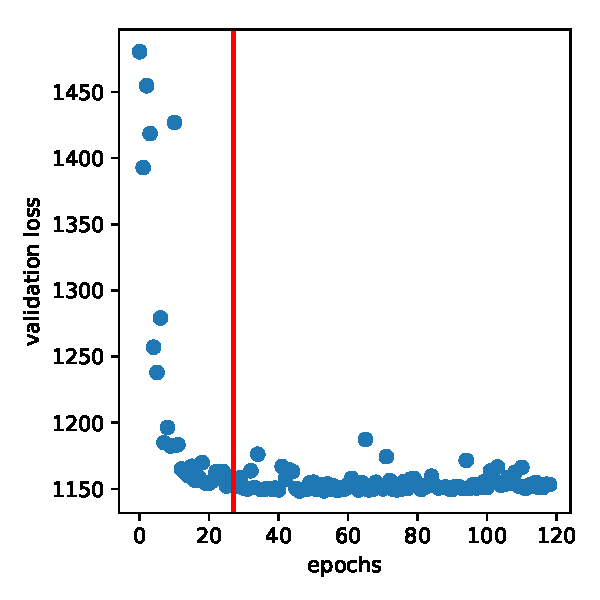
\includegraphics[width=0.49\textwidth]{figures/1M_training_curves.pdf}}
  \hspace{1pt}
  \subfloat{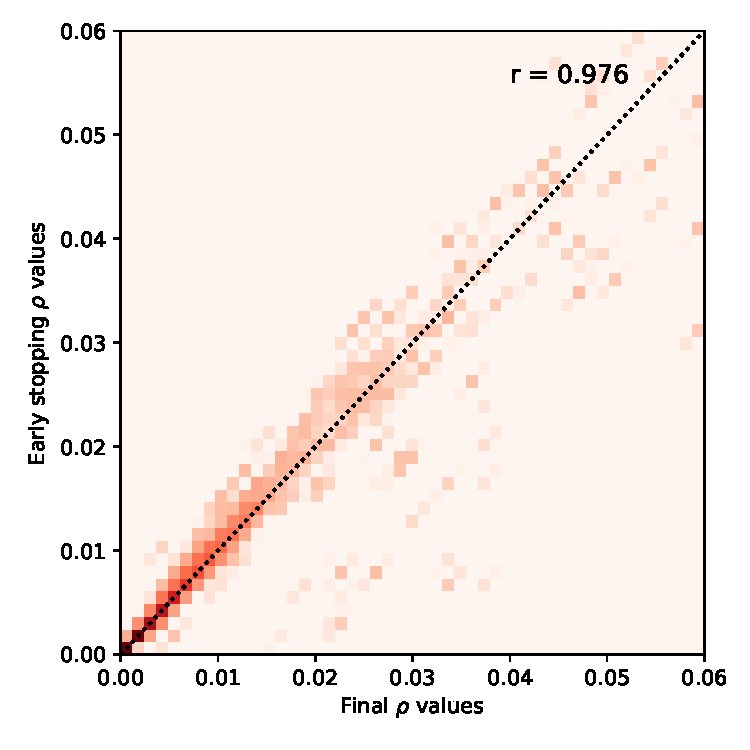
\includegraphics[width=0.49\textwidth]{figures/rho.pdf}}
  \caption[Stability of the early stopping criterion on the one-million-cell sample of the BRAIN-LARGE dataset]{Stability of the early stopping criterion on the one-million-cell sample of the BRAIN-LARGE dataset. (a) Evolution of the loss function ($y$-axis) value on a validation set with the number of epochs ($x$-axis) (b) Contrast of the expected frequency $\rho$-values between the model trained with early stopping ($x$-axis) and the model trained without early stopping ($y$-axis) on a random subset of 100 cells and all genes. We also report the Pearson correlation, $r$.}
\label{scviearly_stopping}
\end{suppfigure}


\begin{suppfigure}[p]
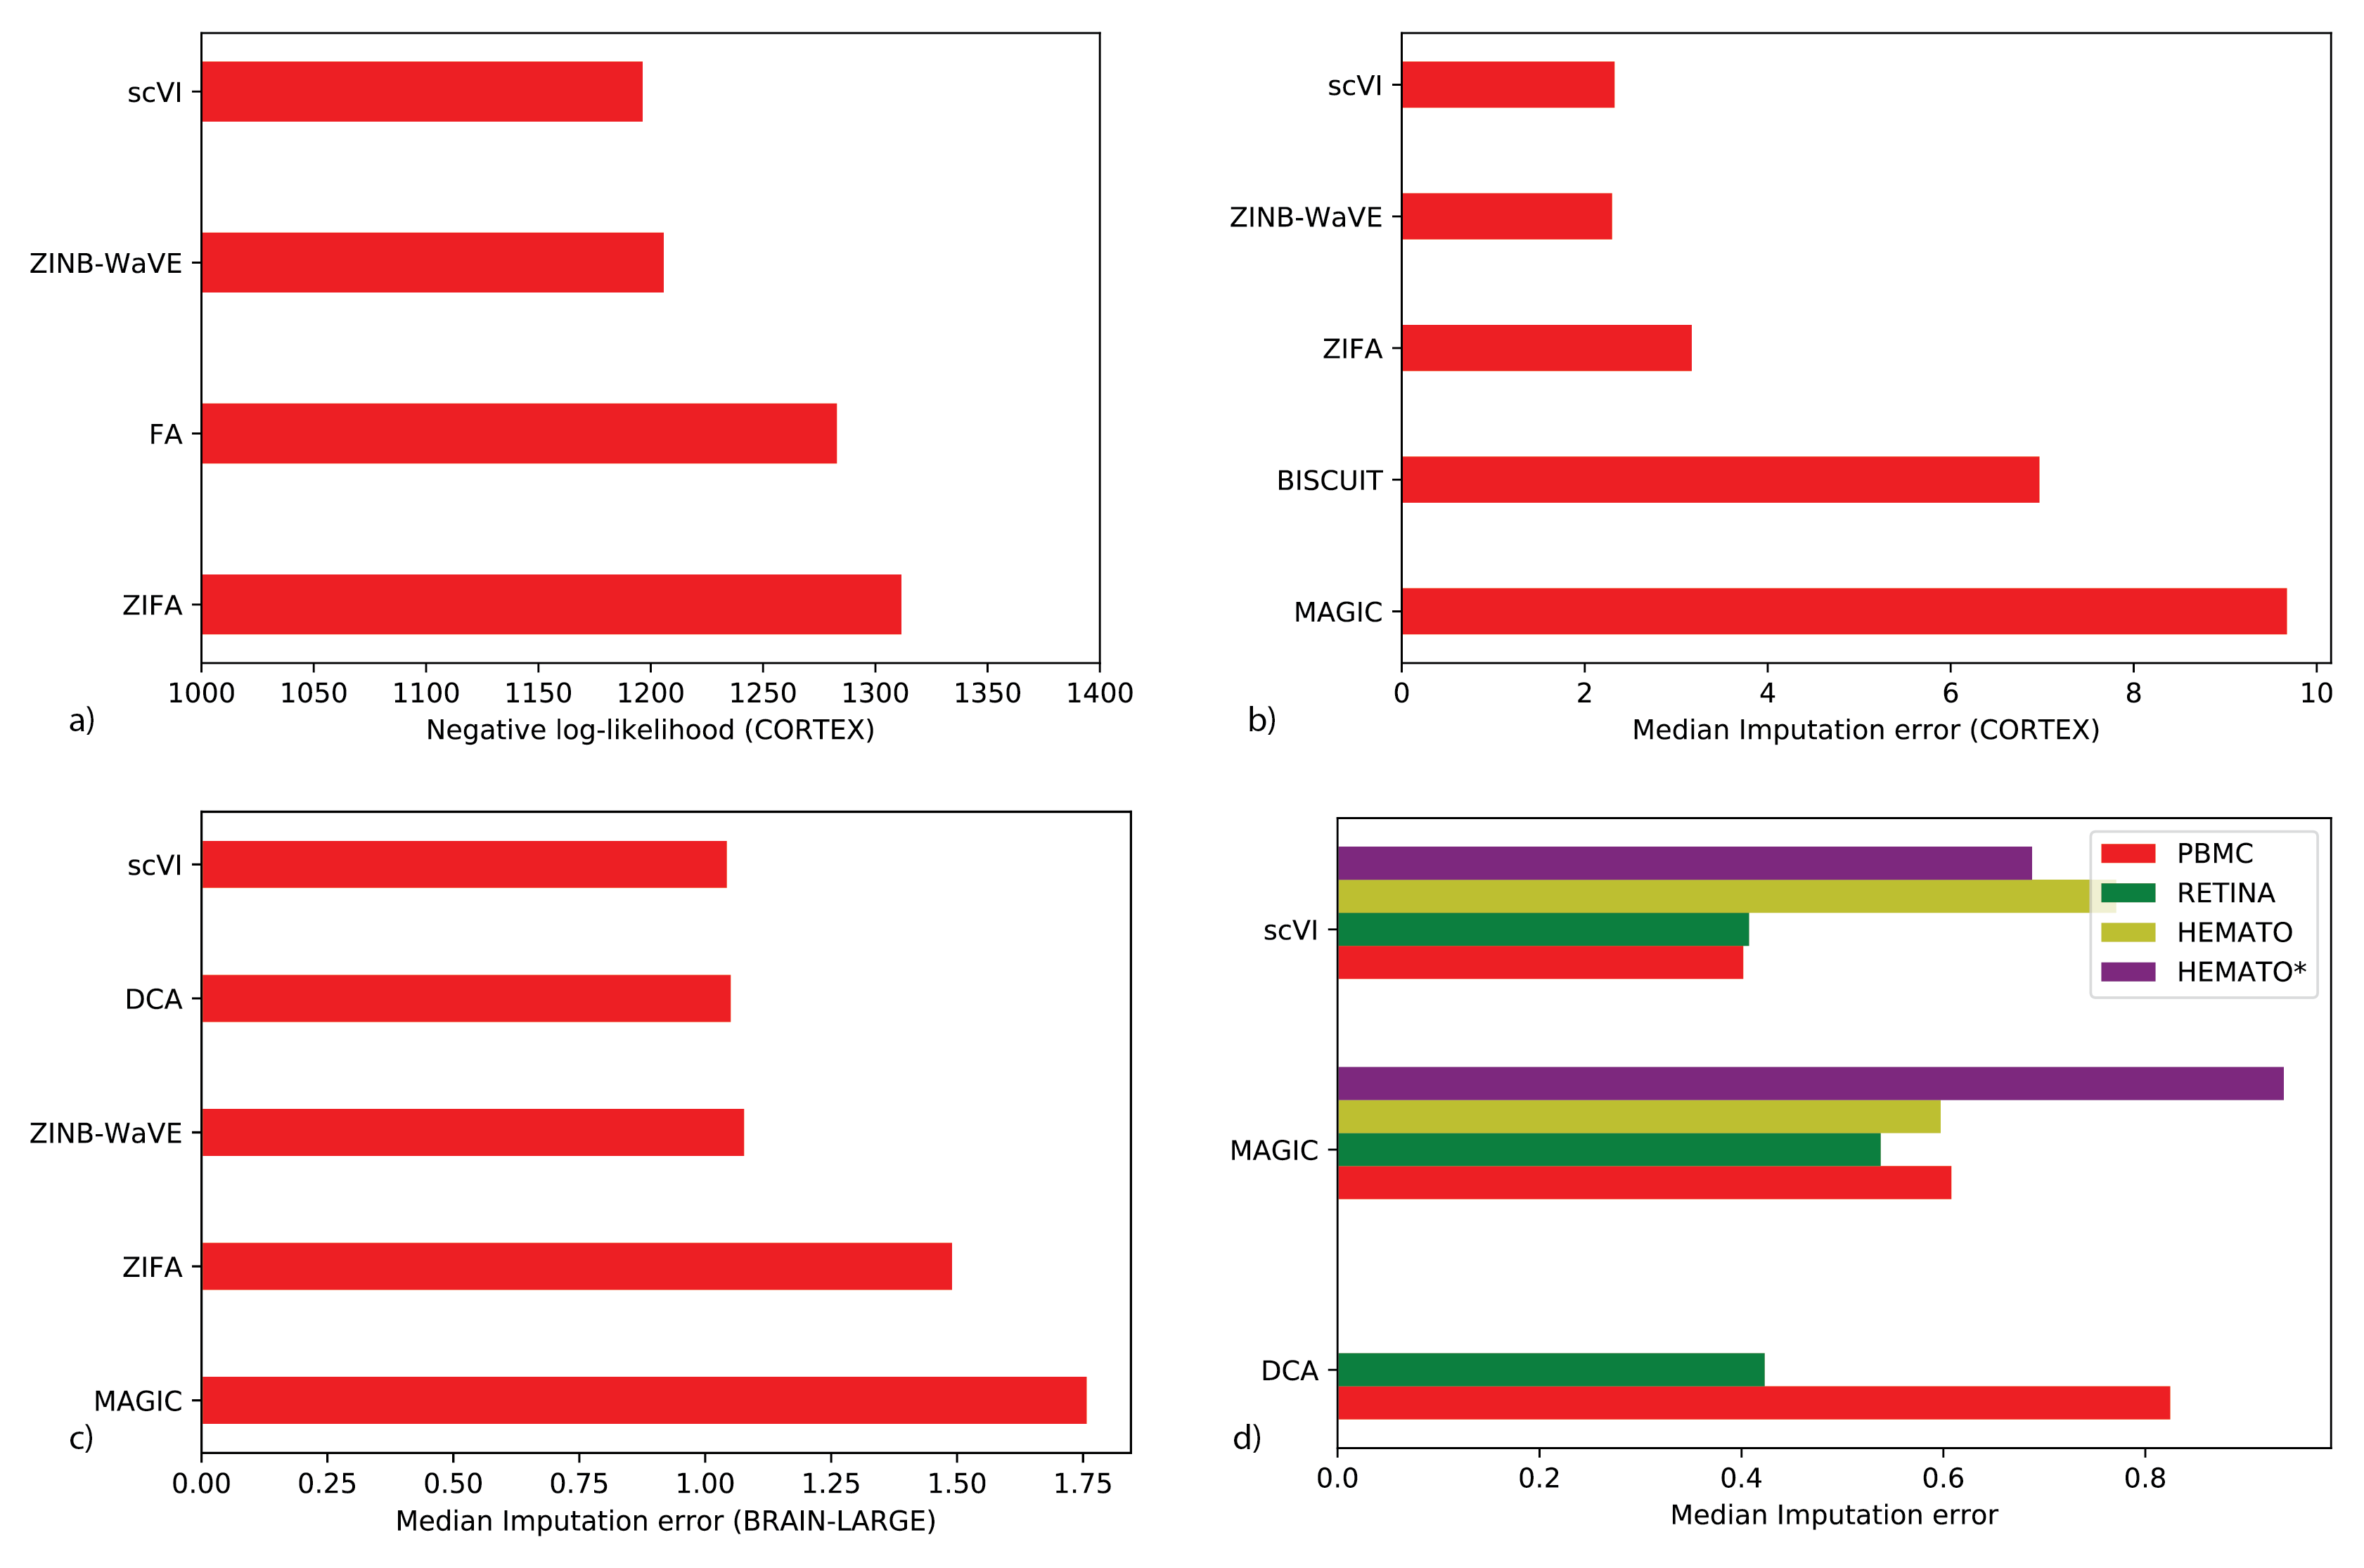
\includegraphics[width=\textwidth]{figures/loglik_imputation_supplement.png}
\caption[Log-likelihood and imputation results]{(a) Log-likelihood results on the CORTEX dataset. (b) through (d): We investigate how scVI latent space can be used to impute the data (with the uniform perturbation scheme) and report benchmarking across datasets for state-of-the-art methods.}
\label{scvilog_imputation_supp}
\end{suppfigure}


\begin{suppfigure}[p]
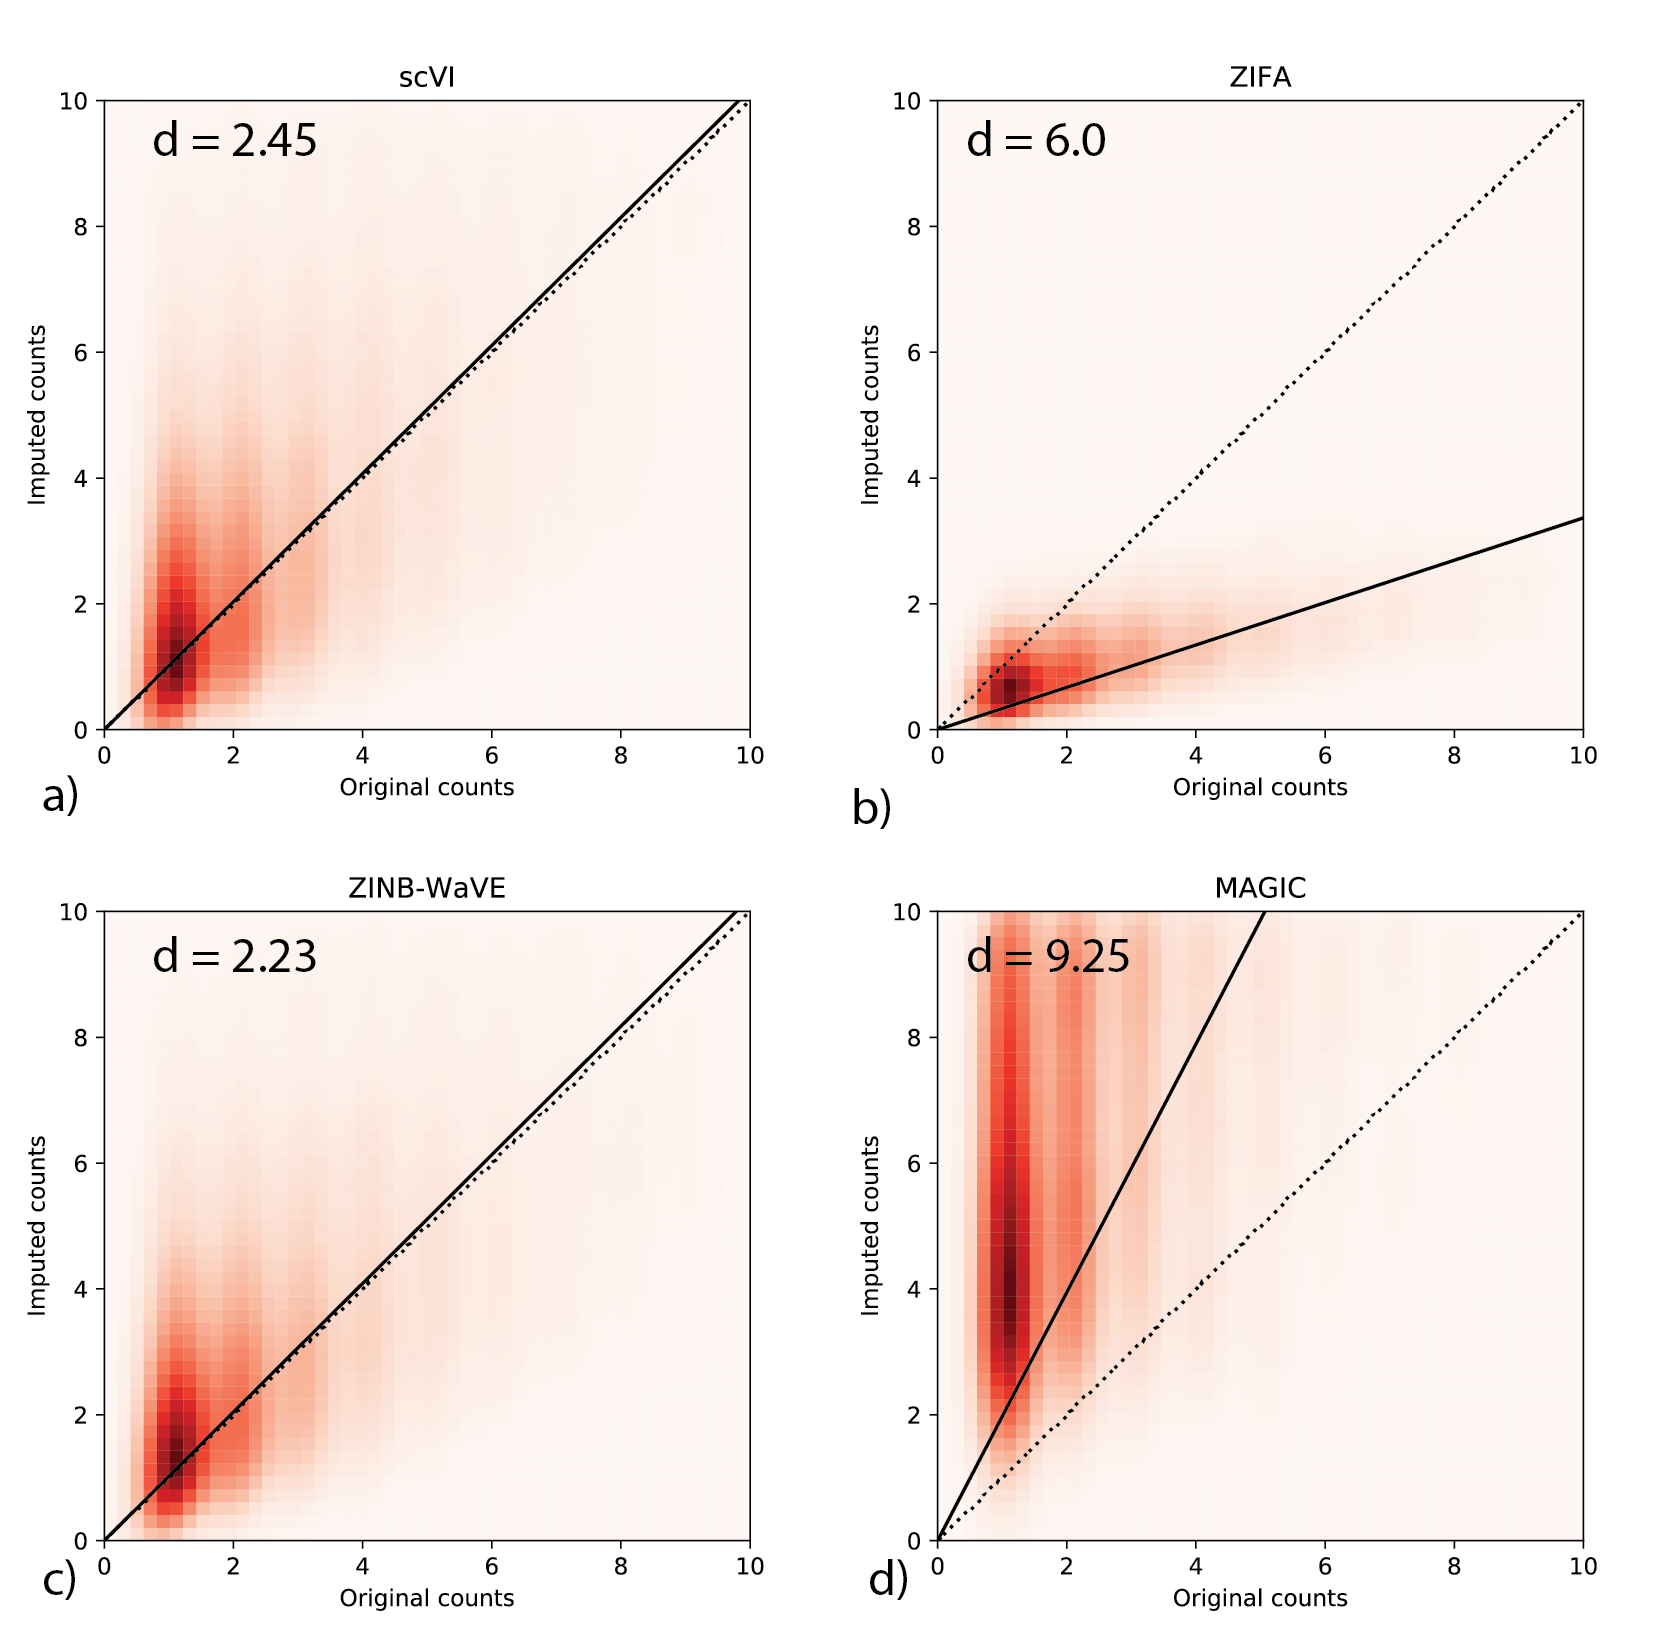
\includegraphics[width=\textwidth]{figures/Figure-3_non_unif.png}
\caption[Non-uniform imputation of scVI on the CORTEX dataset]{Imputation of scVI on the CORTEX dataset. Models are trained on a binomial-down-sampling corrupted dataset (see Methods).  The heatmaps denote density plots of imputed values scVI, ZIFA, MAGIC and ZINB-WaVE on a down-sampled version vs. original values prior to down-sampling. The reported score $d$ is the median imputation error across all the hidden entries (lower is better; see Methods).}
\label{scvilog_imputation_non_unif}
\end{suppfigure}

\begin{suppfigure}[p]
\centering
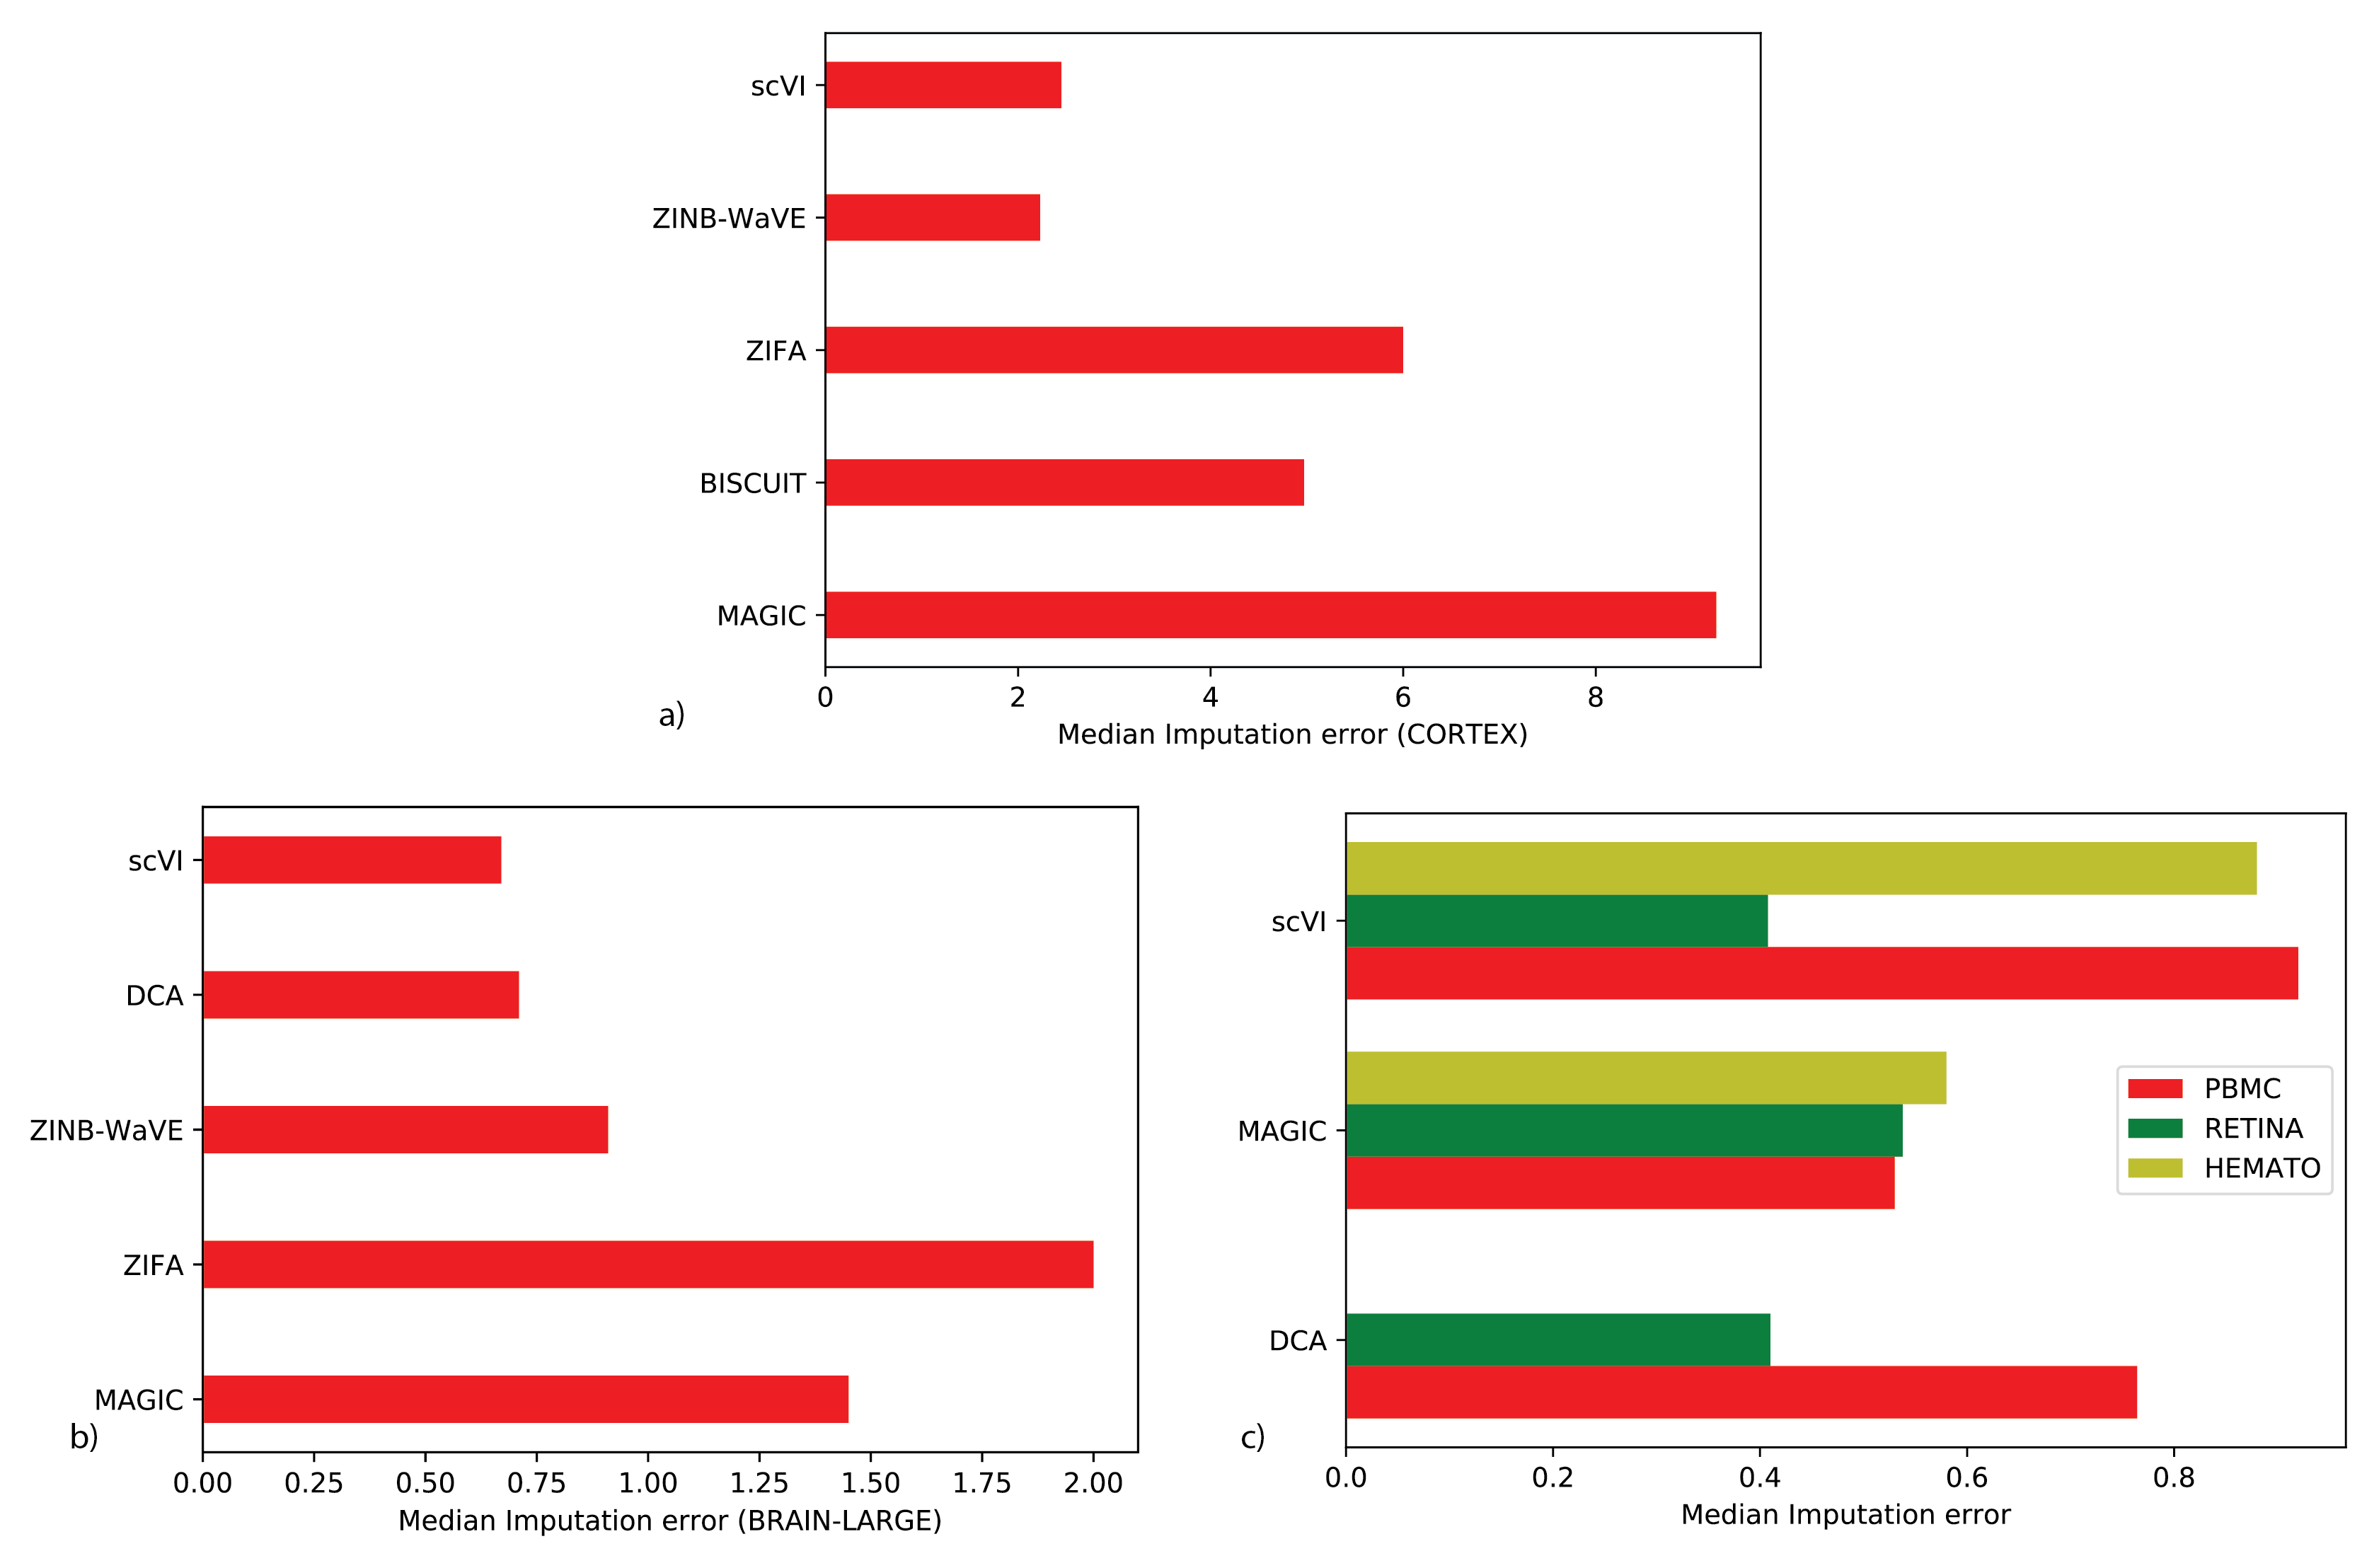
\includegraphics[width=\textwidth]{figures/loglik_imputation_supplement_non_unif.png}
\caption[Non-uniform imputation benchmarking]{(a) through (c): We investigate how scVI latent space can be used to impute the data (with the binomial perturbation scheme) and report benchmarking across datasets for state-of-the-art methods.}
\label{scvilog_imputation_non_unif_supp}
\end{suppfigure}

\begin{suppfigure}[p]
\centering
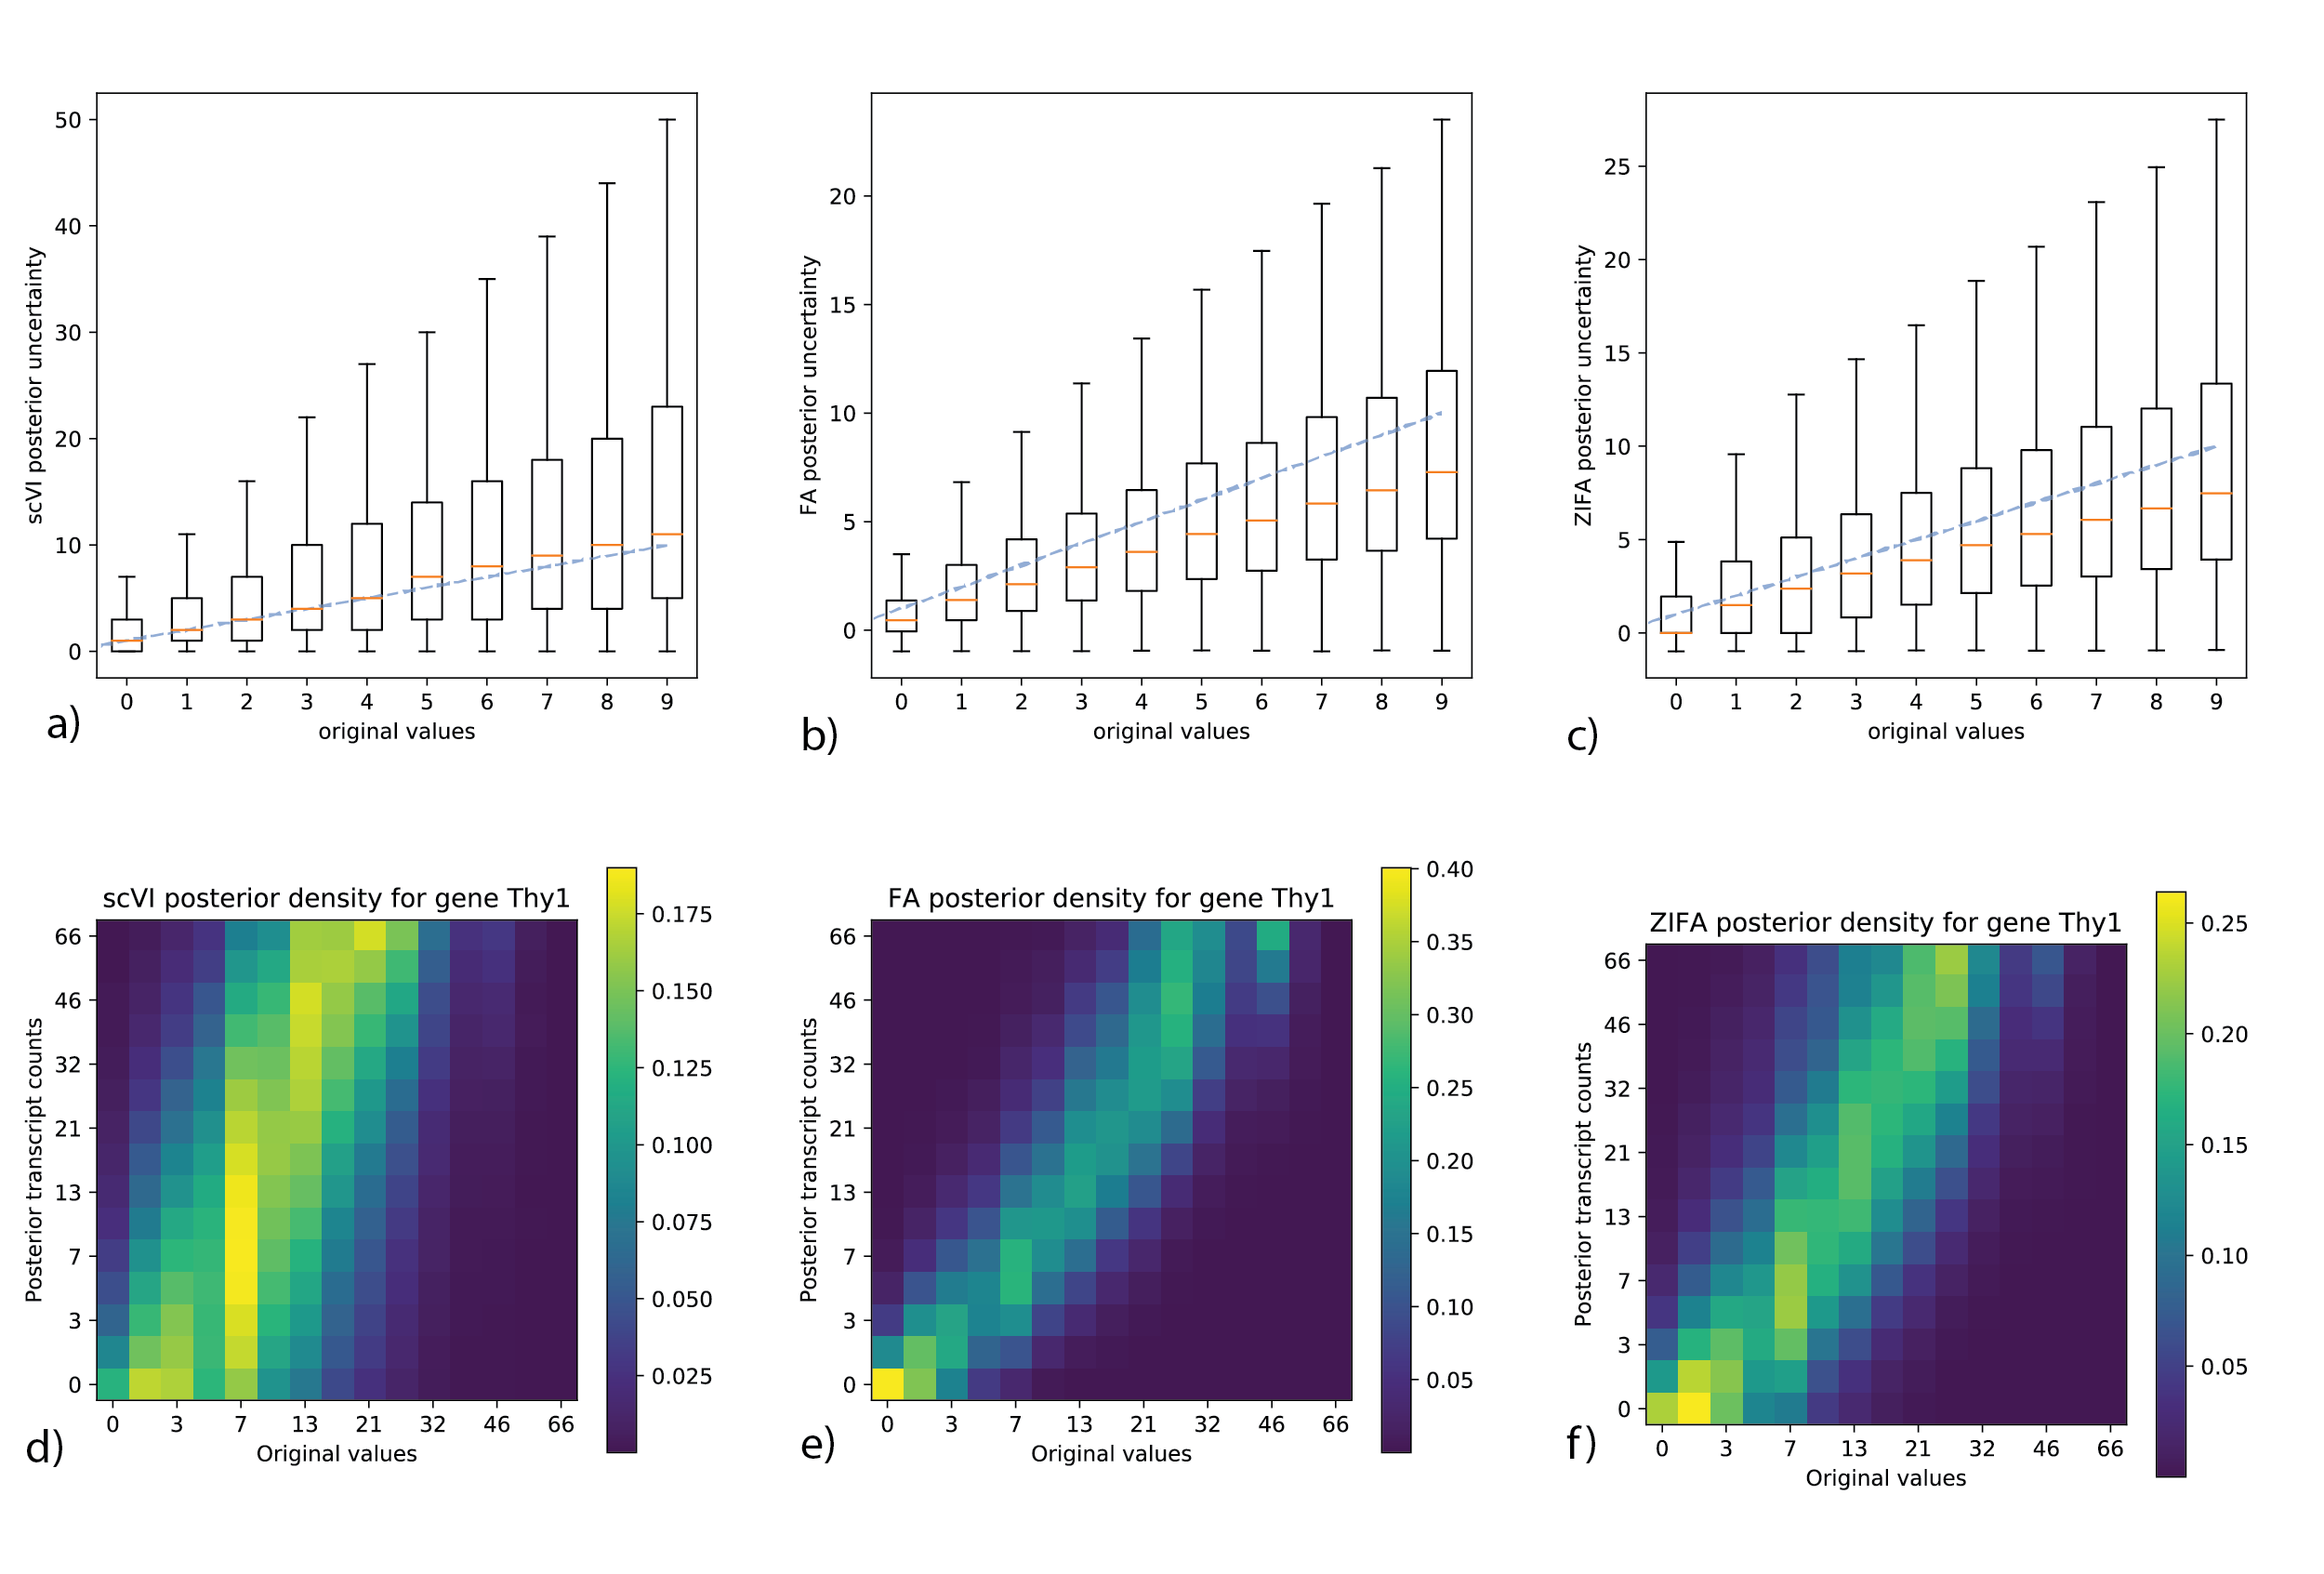
\includegraphics[width=\textwidth]{figures/posterior_supplement.png}
\caption[Posterior analysis of generative models on the CORTEX dataset]{Posterior analysis of generative models on the CORTEX dataset. Panels (a-c) depict the observed counts of randomly selected entries of the data matrix (x-axis) and their posterior uncertainty (y-axis) by sampling from the variational posterior (scVI) or the exact posterior (FA, ZIFA). Whiskers denote the 5th and 95th percentiles. Panels (d-f) represent the observed counts of a representative gene, Thy1, in the CORTEX dataset. Data is presented across all cells ($n=3005$) (x-axis) against the posterior expected counts produced by scVI, ZIFA and FA, respectively (y-axis). The values on each axis have been divided into 20 bins and the color scale reflects the proportion of cells in each pair of bins. By definition, the uncertainty of FA is independent of the input value and tight around the observed count. ZIFA can generate zero and puts realistically more weight in this area. scVI's posterior is more complex, and is able to generate zero for low UMI values but also able to generate high UMI values when the original count observed was only of intermediate intensity.}
\label{scviposterior_supp}
\end{suppfigure}

\begin{suppfigure}
\centering
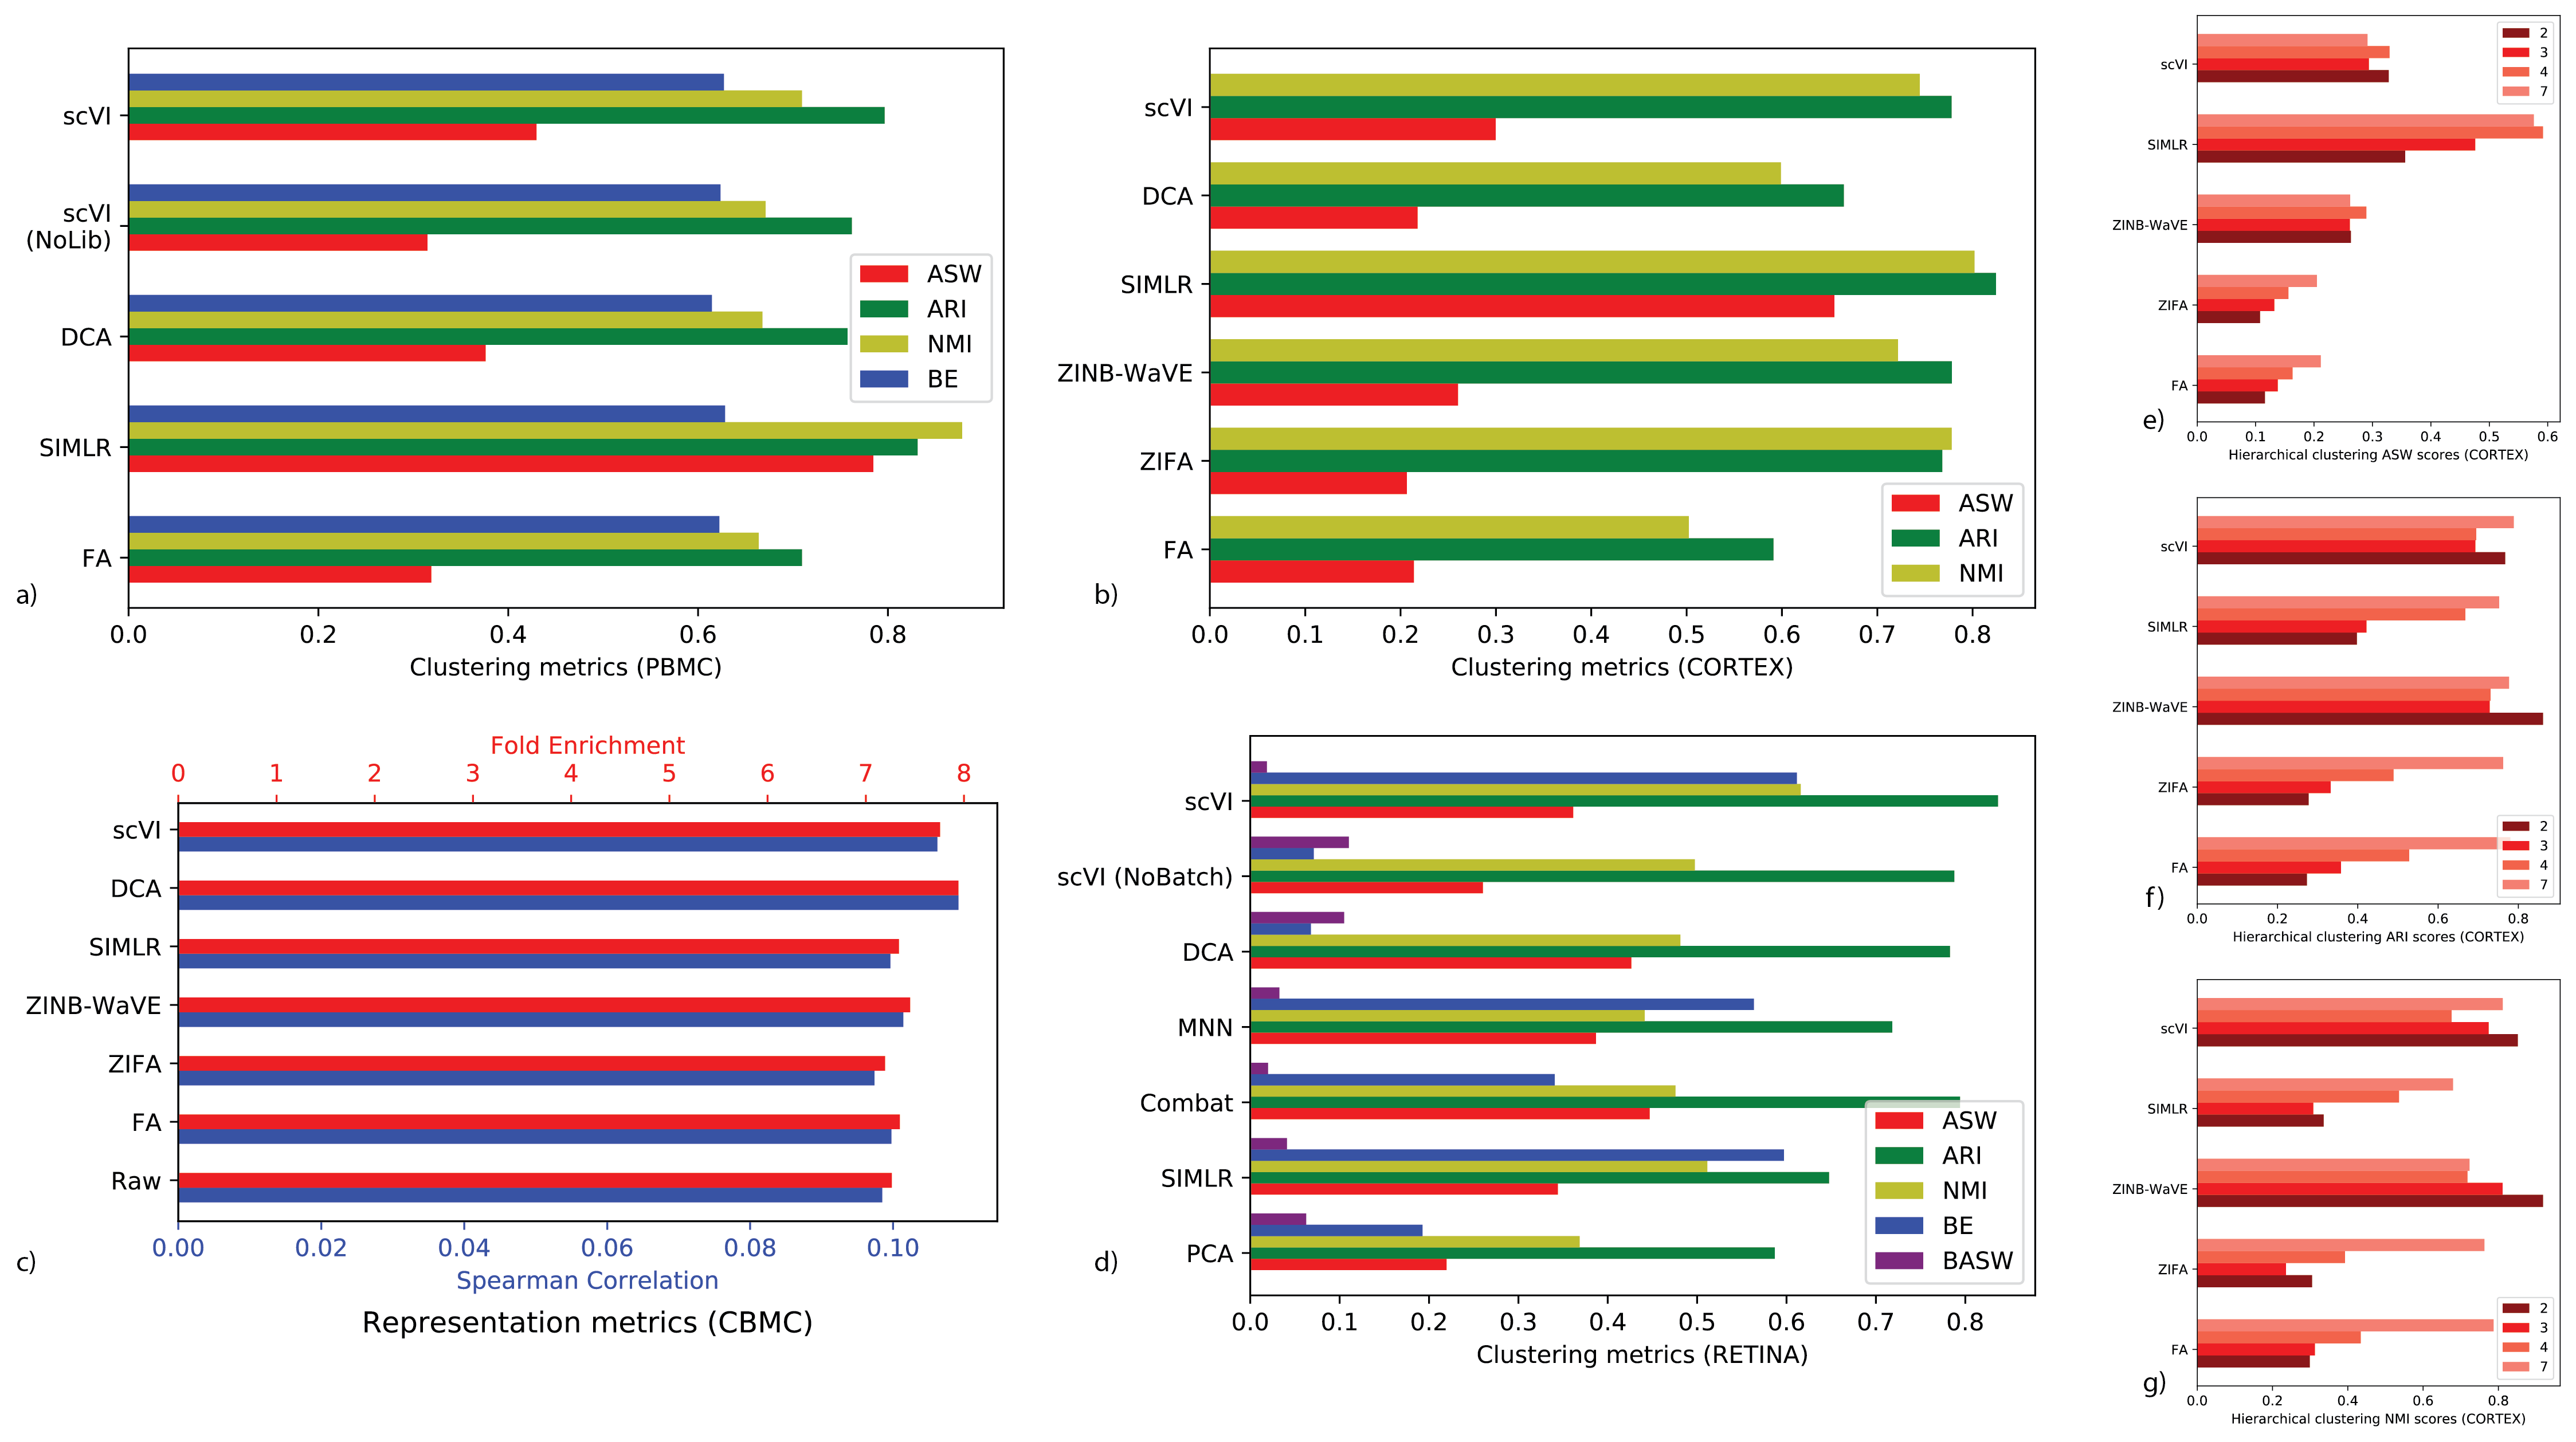
\includegraphics[width=\textwidth]{figures/clustering_supplement.png}
\caption[Clustering performance]{We investigate how scVI latent space can be used to cluster the data and report benchmarking across datasets for state-of-the-art methods. The first four panels depict the results for the (a) PBMC dataset (b) CORTEX (c) CBMC and (d) RETINA. ASW: average silhouette width of pre-annotated subpopulations (higher is better), ARI: adjusted Rand index (higher is better), NMI: normalized mutual information (higher is better), BE: batch-mixing entropy (higher is better), BASW: average silhouette width of batches (lower is better). Panels (e-g) depict the performance of clustering metrics for different depths of the hierarchical clustering in the CORTEX data, computed in the original publication~\cite{Zeisel1138}. The numbers in the legend indicate the number of clusters at the given depth.}
\label{scviclustering_supp}
\end{suppfigure}

\begin{suppfigure}
\centering
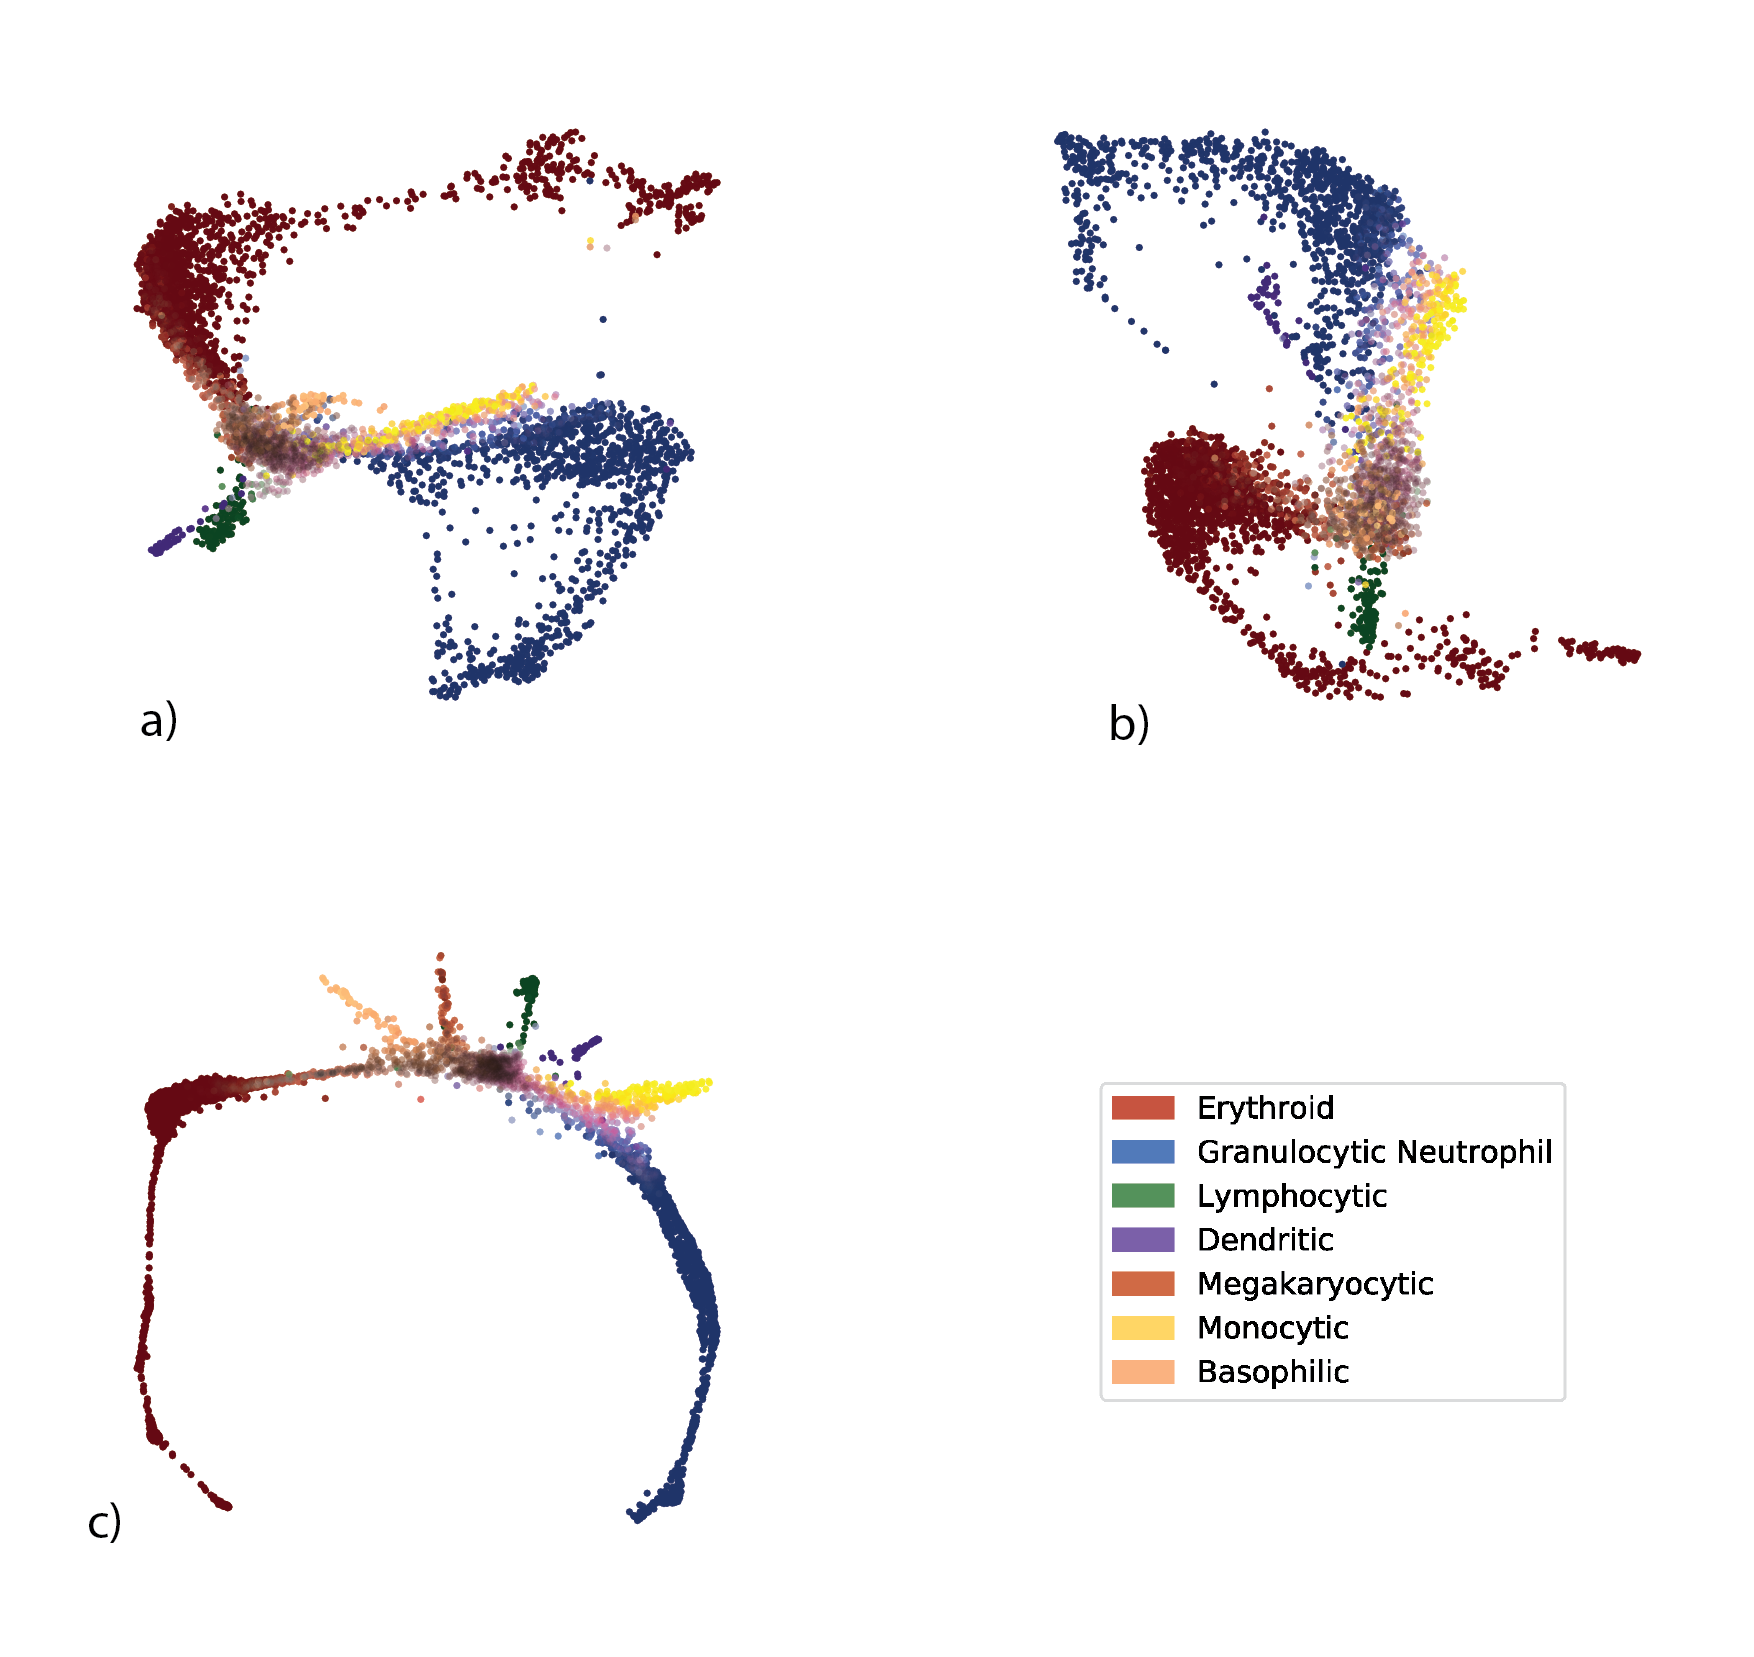
\includegraphics[width=\textwidth]{figures/hemato_supp.png}
\caption[Additional comparison of scVI and PCA on the HEMATO dataset]{Additional comparison of scVI and PCA on the HEMATO dataset. All scatter plots illustrate the embedding of a 5-nearest neighbors graph of a latent space. Cells positions are computed using a force-directed layout; (a) denotes a reduction to 60 pcs as in the original paper. (b) denotes the output of a scVI in dimension 60. As the dimension is sensibly different from other experiments, the warm-up schedule (which governs how the prior on $z$ is enforced) was adjusted. (c) denotes the figure from the main paper. To recover all the differentiation paths, the authors performed several operations on the $K$-nearest neighbors graph that we did not reproduce in this analysis. We instead visualize the graph before the smoothing procedure.}
\label{scvihemato_supp}
\end{suppfigure}


\begin{suppfigure}
\centering
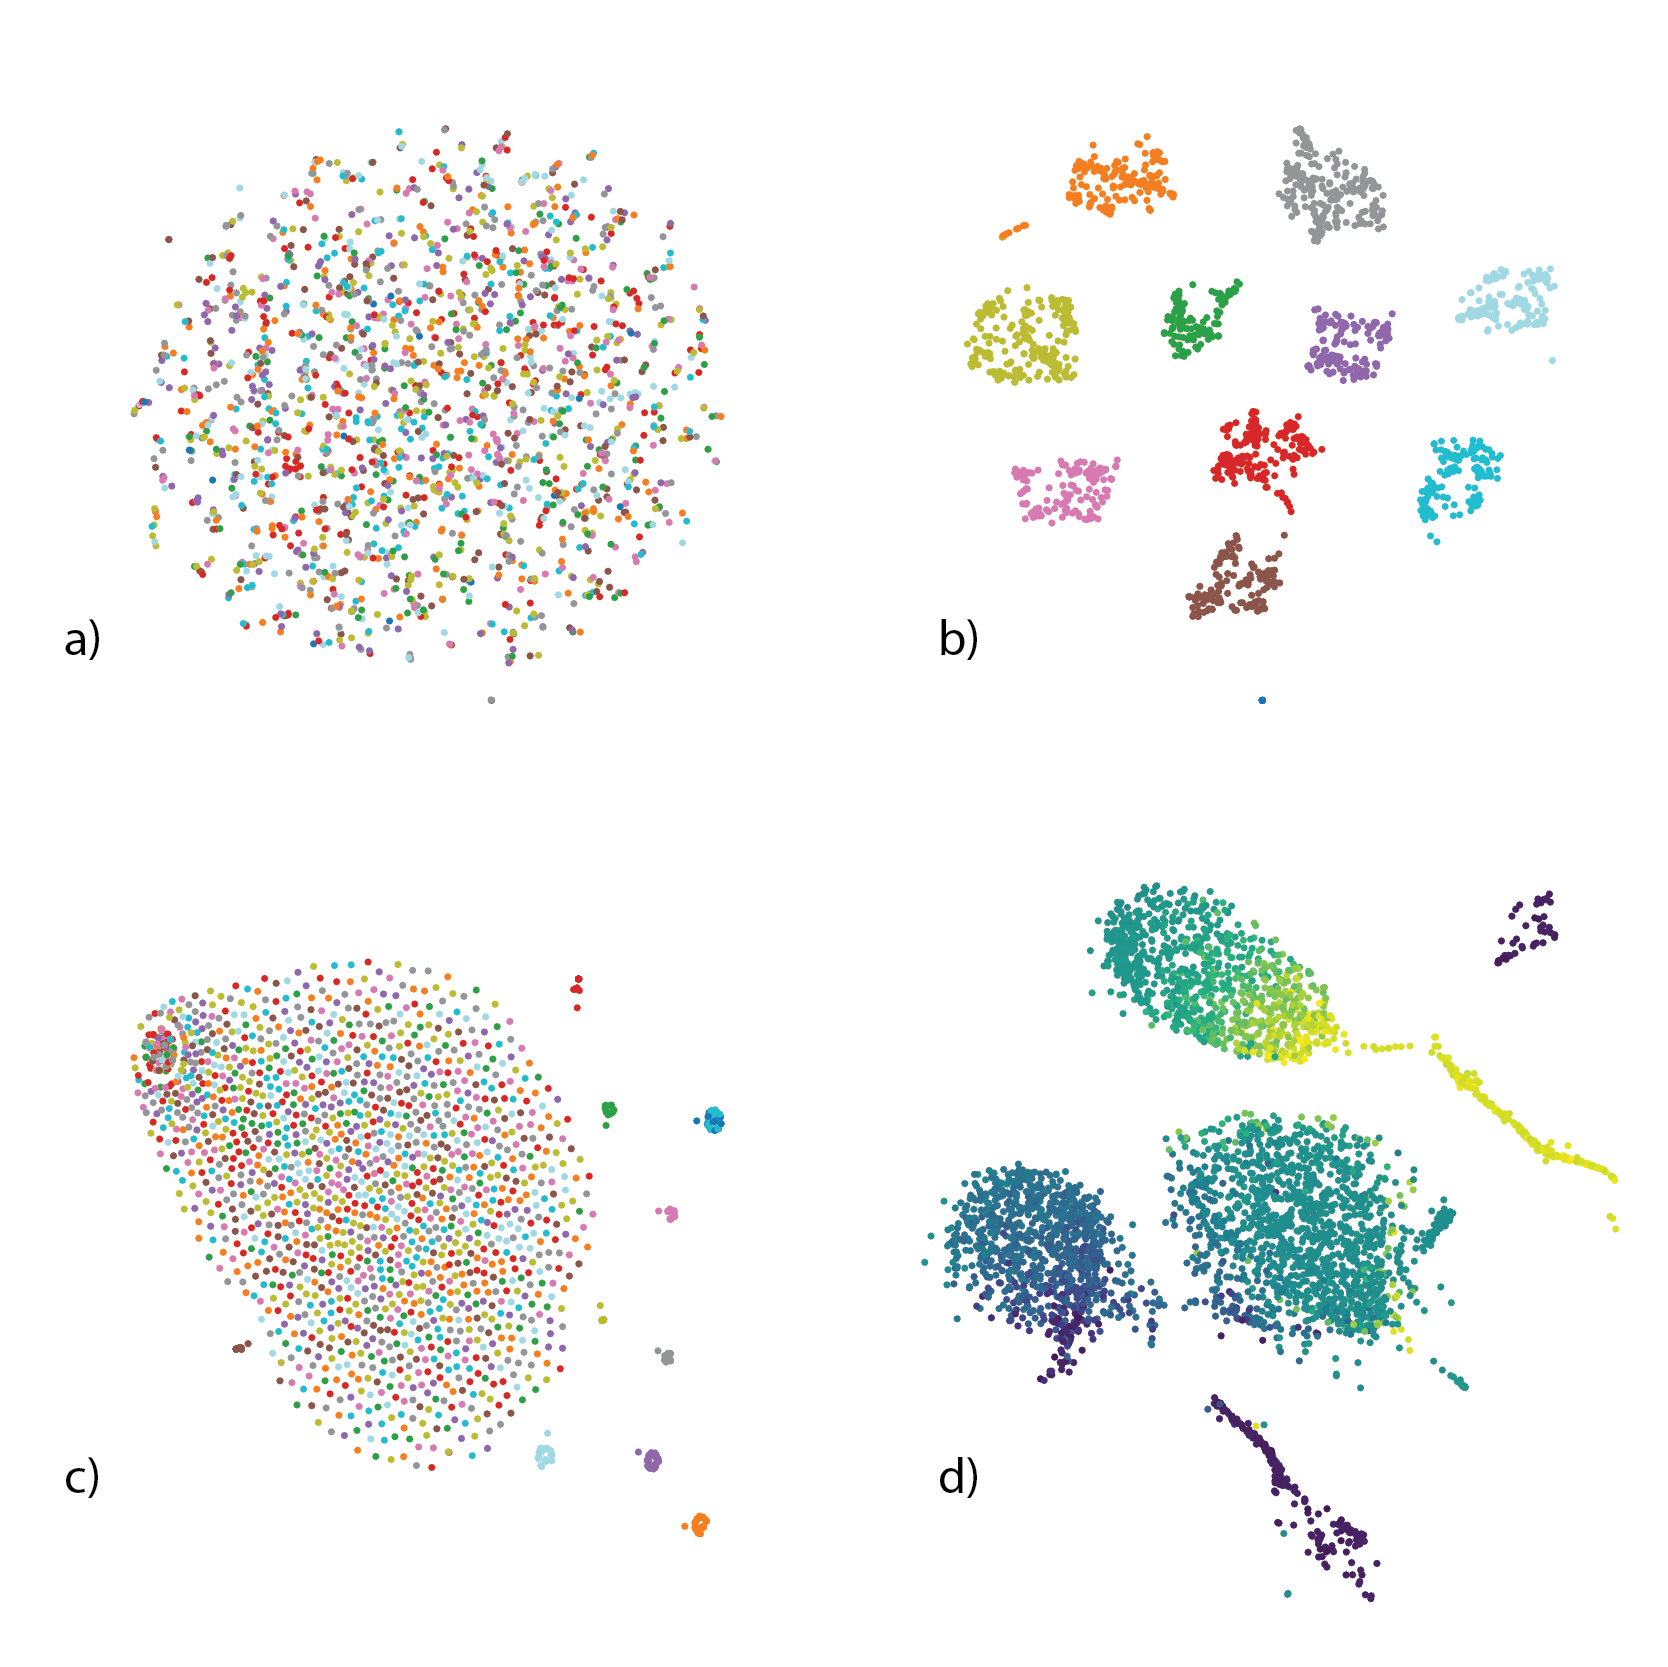
\includegraphics[width=\textwidth]{figures/SIMLR_supplement.png}
\caption[Details for the clustering panel]{Details for the clustering panel. For the random data, we obtain the labels that order the cell-cell similarity matrices by a k-means clustering on SIMLR latent space. (a) scVI latent space with SIMLR labels. There is no structure. (b) SIMLR latent space with SIMLR labels. (c) PCA latent space with SIMLR labels. (d) SIMLR tSNE on the HEMATO dataset. We prefer to visualize the SIMLR embedding on a kNN graph since the continuum structure of the dataset would be lost, even with tSNE.}
\label{scvisuppfig2}
\end{suppfigure}


\begin{suppfigure}[htp]
  \centering
  \begin{subfigure}[b]{0.3\textwidth}
        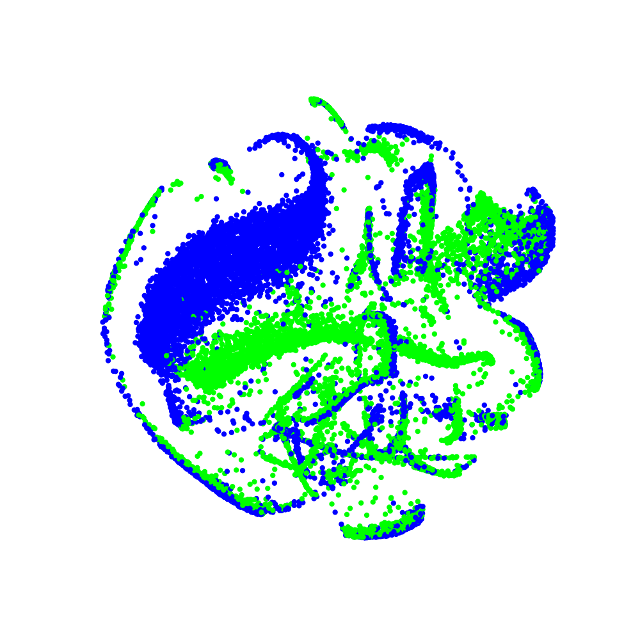
\includegraphics[width=\textwidth]{figures/PCA_tSNE_bipolar_batch.png}
        \caption{tSNE embedding for PCA, colored by batch}
    \end{subfigure}
\hspace{5pt}
  \begin{subfigure}[b]{0.3\textwidth}
        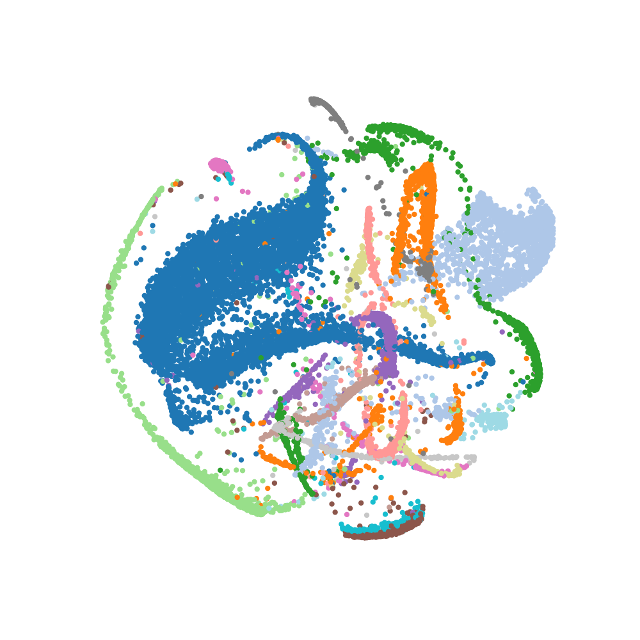
\includegraphics[width=\textwidth]{figures/PCA_tSNE_bipolar_clusters.png}
        \caption{tSNE embedding for PCA, colored by cell type}
    \end{subfigure}
  \hspace{5pt}
    \begin{subfigure}[b]{0.3\textwidth}
        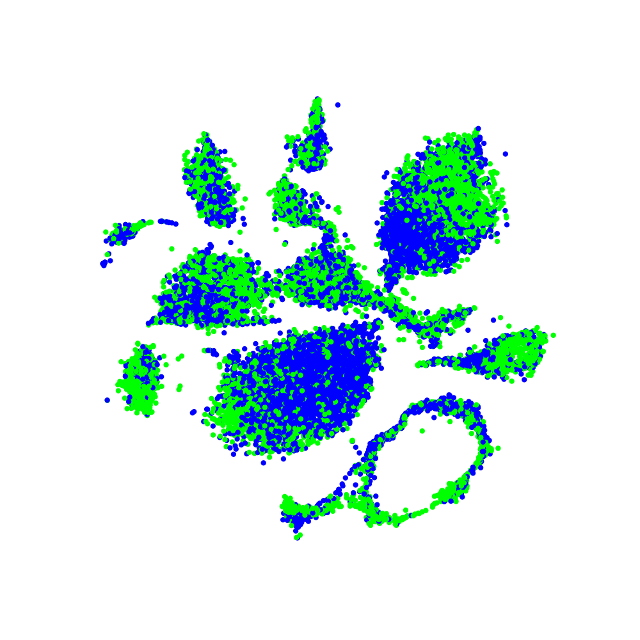
\includegraphics[width=\textwidth]{figures/SIMLR_tSNE_bipolar_batch.png}
        \caption{Embedding for SIMLR, colored by batch}
    \end{subfigure}
  \hspace{5pt}
      \begin{subfigure}[b]{0.3\textwidth}
        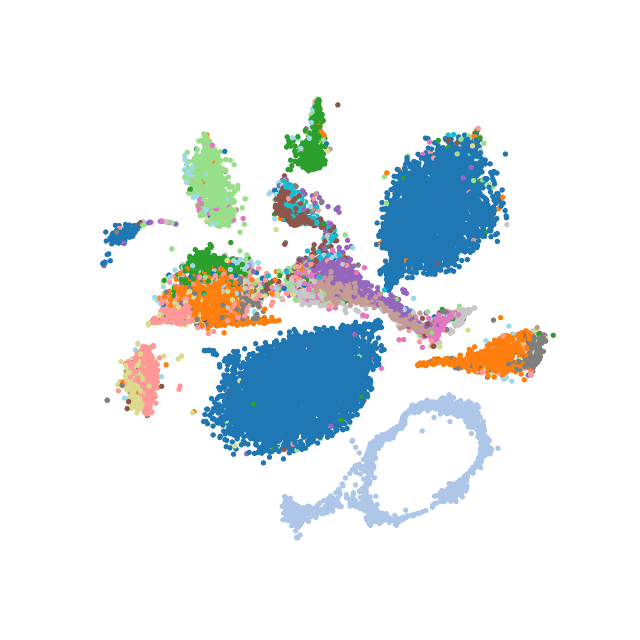
\includegraphics[width=\textwidth]{figures/SIMLR_tSNE_bipolar_clusters.png}
        \caption{Embedding for SIMLR, colored by cell type}
    \end{subfigure}
  \hspace{5pt}
      \begin{subfigure}[b]{0.3\textwidth}
        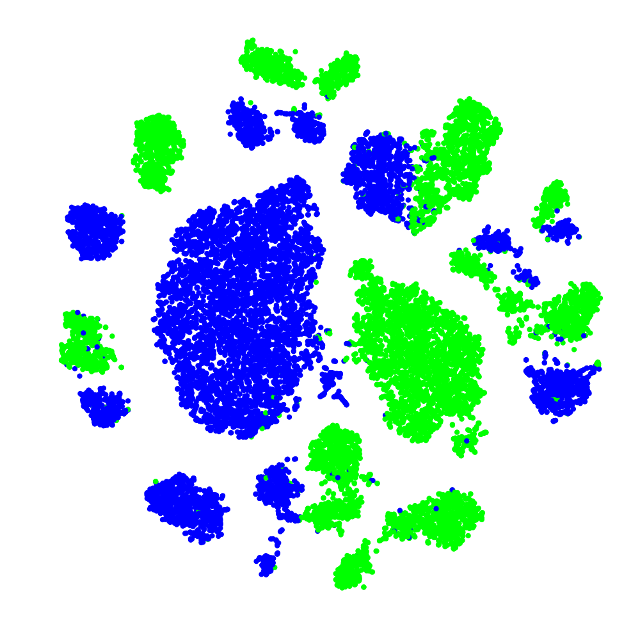
\includegraphics[width=\textwidth]{figures/DCA_tSNE_bipolar_batch.png}
        \caption{Embedding for DCA, colored by batch}
    \end{subfigure}
  \hspace{5pt}
      \begin{subfigure}[b]{0.3\textwidth}
        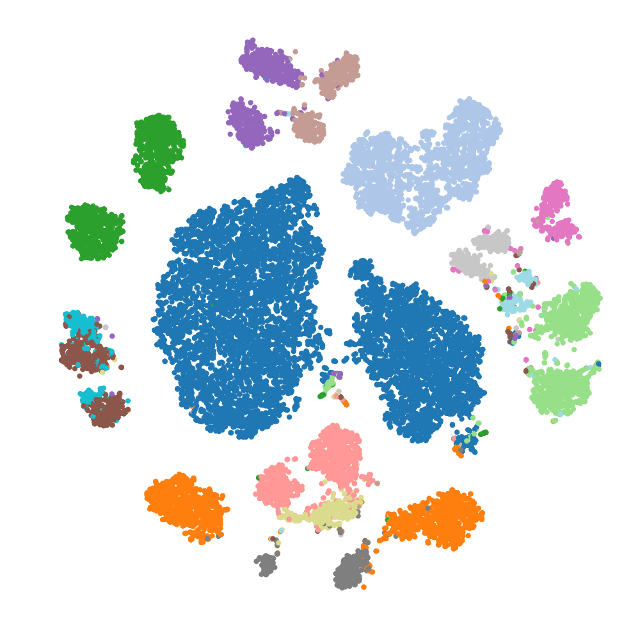
\includegraphics[width=\textwidth]{figures/DCA_tSNE_bipolar_clusters.png}
        \caption{Embedding for DCA, colored by cell type}
    \end{subfigure}
  \caption[Batch effect removal on the RETINA dataset]{Batch effect removal on the RETINA dataset. (a, b) Embedding plots for PCA were generated by applying tSNE on the respective latent space. (c, d) For SIMLR, we used the tSNE coordinates provided by the program and the number of clusters was set to the number of pre-annotated subpopulations ($n=15$). (e, f) Embedding plots for DCA were generated by applying tSNE on the respective latent space.}
  \label{scviMNNfigure}
\end{suppfigure}


\begin{suppfigure}
\centering
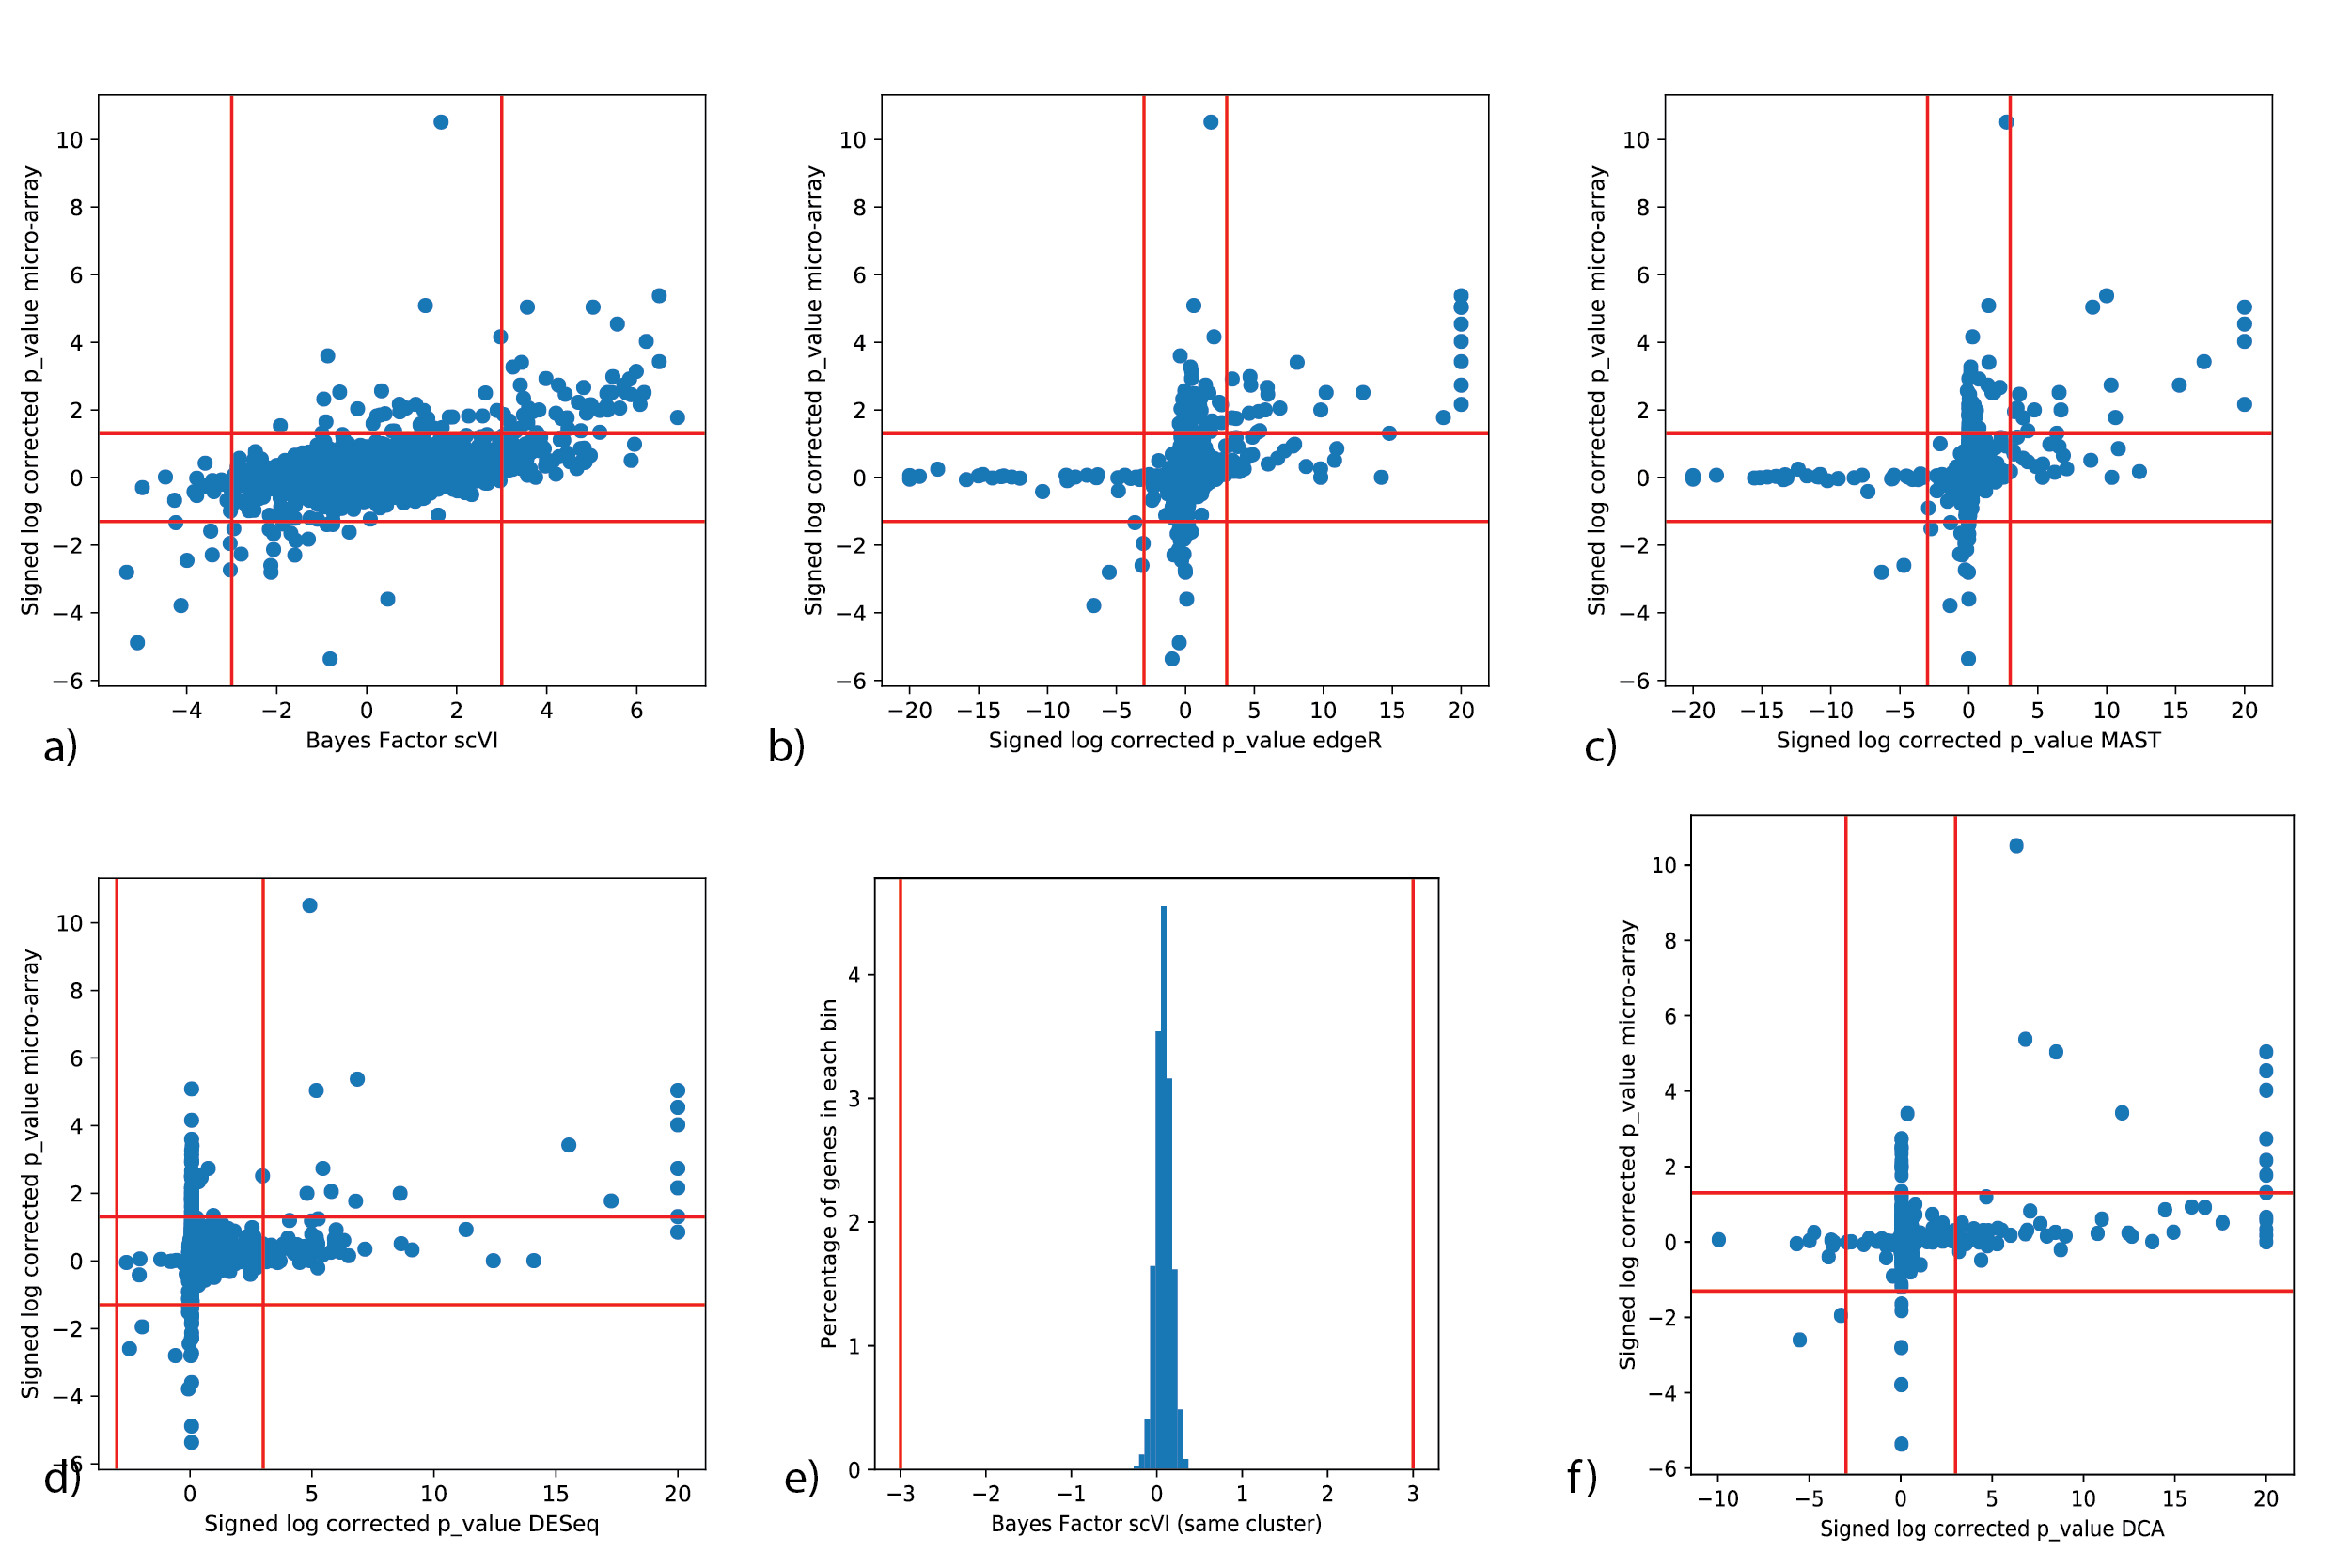
\includegraphics[width=\textwidth]{figures/de_figure.png}
\caption[Differential expression with scVI on the PBMC dataset]{Differential expression with scVI on the PBMC dataset. (a) (b) (c) (d) (f) p-values of microarray against p-values or Bayes factor for CD4 /CD8 comparison. In the order indicated, scVI, edgeR, MAST, DESeq2, DESeq2 on DCA imputed counts (e) Bayes factor of scVI when applying DE to two sets of random cells from the same cluster.}
\label{scvibayes_supp}
\end{suppfigure}

\begin{suppfigure}
\centering
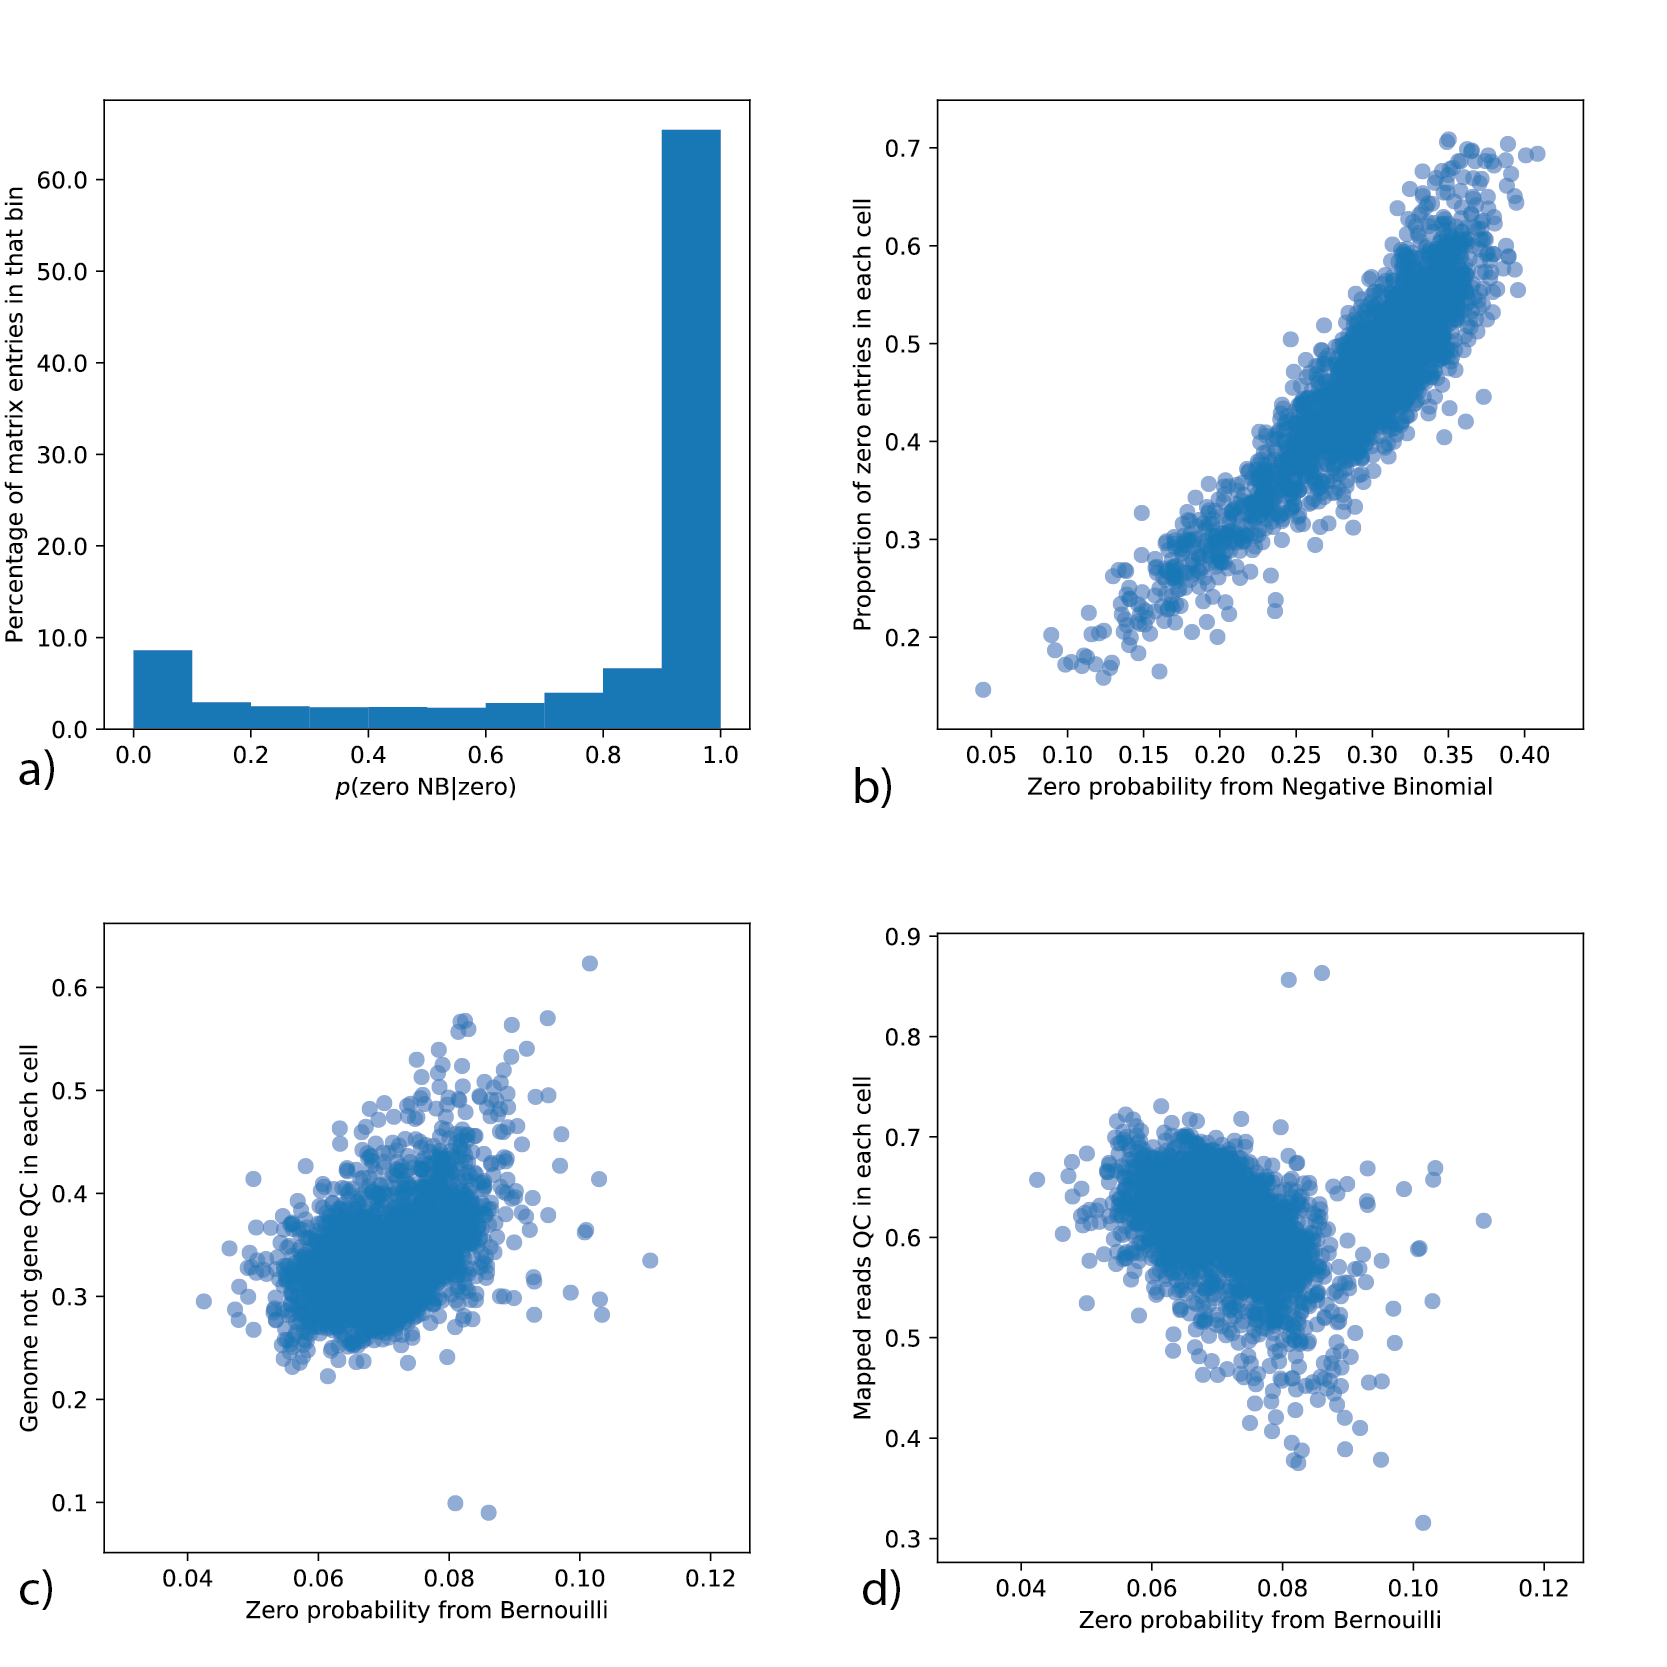
\includegraphics[width=\textwidth]{figures/parameter_supplement.png}
\caption[The generative distributions of scVI]{The generative distributions of scVI. This study focuses on a particular subpopulation of the BRAIN-SMALL dataset  ($n=2592$)
(a) To assess whether most of the zeros in the data comes from the negative binomial, for each entry of the count matrix (percentage in y-axis), we plot the probability that a given zero comes from the NB conditioned on having a zero (x-axis).
(b) Number of genes detected vs. negative binomial zero probability averaged across all genes.
(c) Genome\_not\_gene vs. Bernoulli zero probability averaged across all genes.
(d) Mapped\_reads vs. Bernoulli zero probability averaged across all genes. }
\label{scviparameters_supp}
\end{suppfigure}

\begin{suppfigure}
\centering
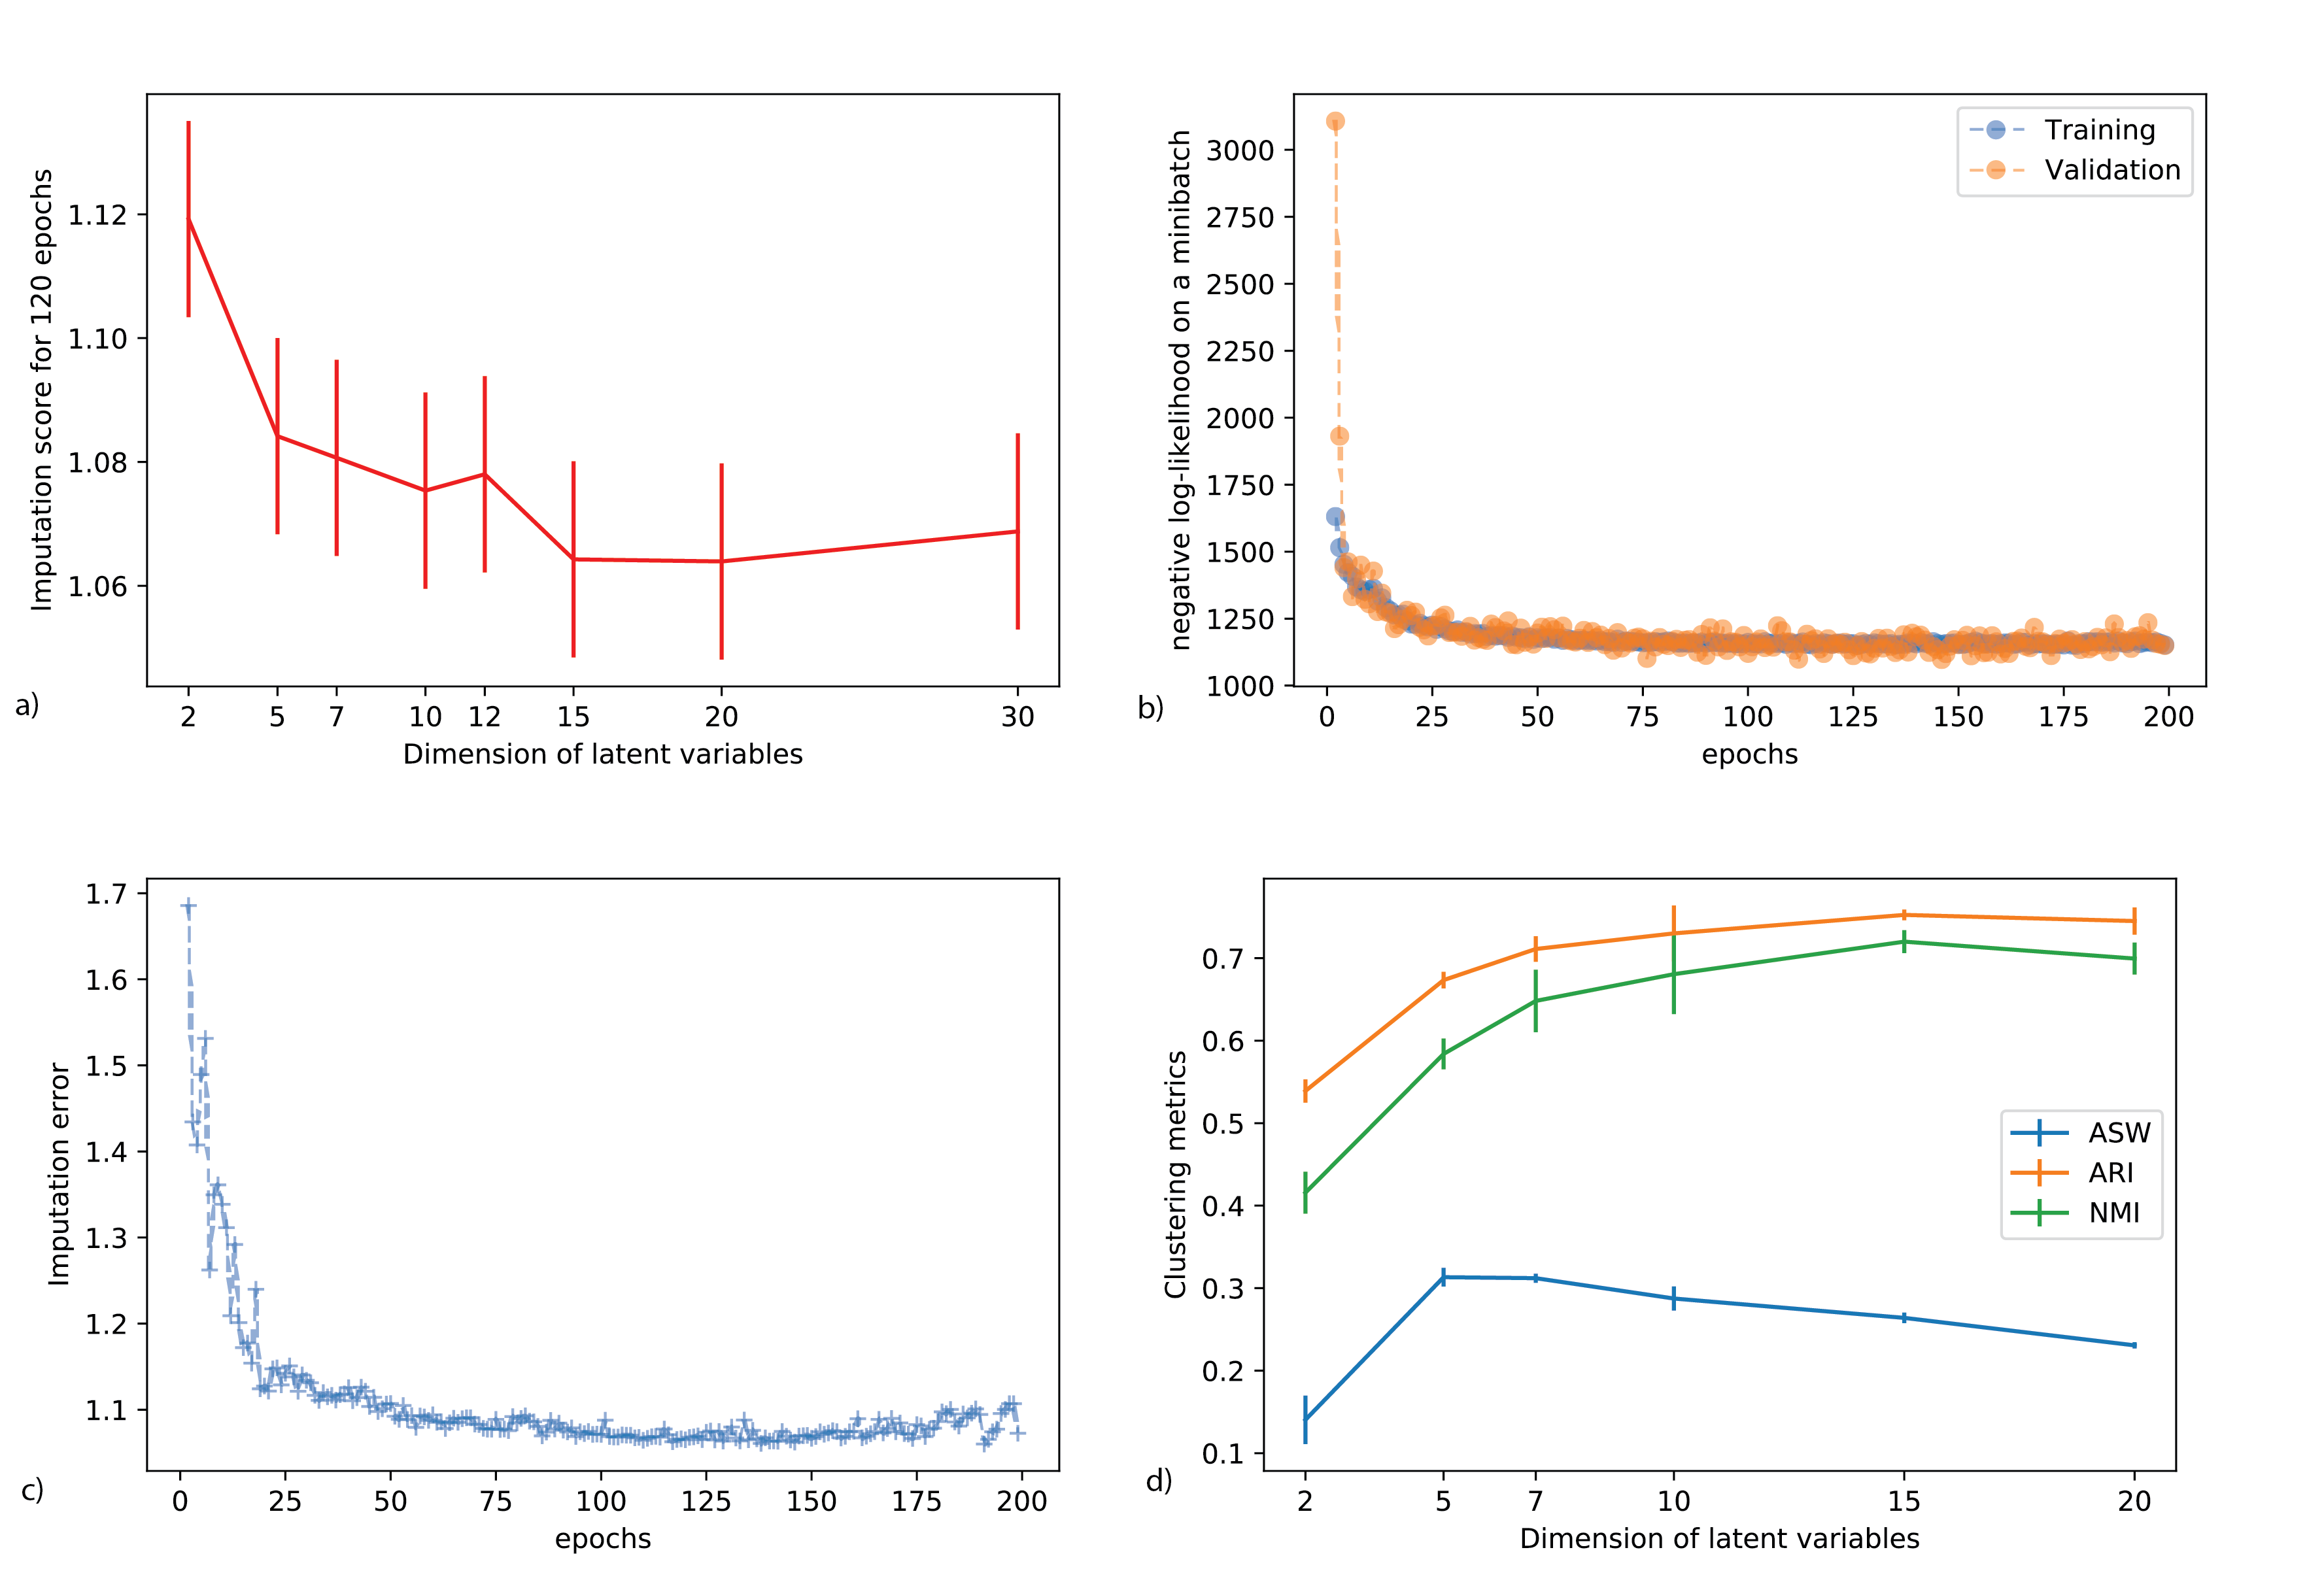
\includegraphics[width=\textwidth]{figures/stability_figure.png}
\caption[Robustness analysis for scVI]{Robustness analysis for scVI. Whiskers denote 5th and 95th percentiles. (a) Imputation score on the BRAIN-LARGE dataset across multiple random initialization, training and dimension of the latent space. (b) Visualization of scVI numerical objective function during training on the BRAIN-LARGE dataset. This shows our model does not over fit and has a stable training procedure. (c) Imputation score as a function of the number of epochs on the BRAIN-LARGE dataset. This figure also shows stability across posterior sampling since there is not much change in the parameters between two subsequent epochs. (d) Clustering metrics on the CORTEX dataset across multiple initializations and dimensions for the latent space.}
\label{scvirobustness}
\end{suppfigure}


